% TEXINPUTS=.:tikzuml-v*: pdflatex abrt.tex
\documentclass{article}
\usepackage[utf8]{inputenc}
\usepackage[english]{babel}
\usepackage[usenames,dvipsnames]{xcolor}
\usepackage{tikz}
\usetikzlibrary{arrows,shapes,mindmap,shadows,positioning}
\usepackage{hyperref}
\usepackage{fullpage}
\usepackage{graphicx}
\usepackage{fancybox}
\usepackage{tikz-uml}

% The document is based on a template from project management book "A
% Guide to the Project Management Body of Knowledge" (PMBOK Guide).

\title{ABRT Project Document}
\author{Karel Klíč}

\begin{document}
\maketitle

ABRT improves quality of operating systems by automatic detection of
software failures, their analysis on a centralised server, and
reporing failures to the right group of developers.  It is designed to
help users to report problems, help developers to fix the bugs found
in the reports, help security engineers to determine the security
impact of a failure, and help quality assurance and release
engineering people to assess the overall quality of an operating
system release.

This is a top-level project document for ABRT.  It describes the
top-level design, communication protocols and interfaces.  It also
describes the current status of the features, and project roadmap.

\paragraph{Contributors.}  Miroslav Lichvár contributed figures
\ref{fig:cumulative} and \ref{fig:distribution}.  Miroslav Lichvár and
Michal Toman co-designed the database schema for the Problem Storage.
Jiří Moskovčák co-designed the use cases.  Jon McCann designed the
graphical user interface of the client.

\cleardoublepage
\tableofcontents

\cleardoublepage
\section{Project Charter}

\subsection{Statement of Work}

business need, product scope, strategic plan

\subsection{Business case}

\subsubsection{Enterprise Client-Side Use Case 1}

\begin{tikzpicture}
\umlactor[x=-4,y=0]{End User}
\umlactor[x=6,y=0]{Support Portal}
\begin{umlsystem}[x=1,fill=red!10]{ABRT Client}
\umlusecase[x=0,y=2.4]{Send a $\mu$Report}
\umlusecase[x=0,y=0.8]{Read an Advice}
\umlusecase[x=0,y=-0.8]{Send a Full Report}
\umlusecase[x=0,y=-2.4]{Open a New Case}
\end{umlsystem}
\umlassoc{End User}{usecase-1}
\umlassoc{End User}{usecase-2}
\umlassoc{End User}{usecase-3}
\umlassoc{End User}{usecase-4}
\umlassoc{Support Portal}{usecase-1}
\umlassoc{Support Portal}{usecase-2}
\umlassoc{Support Portal}{usecase-3}
\umlassoc{Support Portal}{usecase-4}
\end{tikzpicture}

\subsubsection{Enterprise Client-Side Use Case 2}

\begin{tikzpicture}
\umlactor[x=-6,y=0]{End User}
\umlactor[x=10,y=0]{Administrator}
\umlactor[x=10,y=-3]{Support Portal}
\begin{umlsystem}[x=1,fill=red!10]{ABRT Server}
\umlusecase[x=-2,y=2,name=send microreport]{Send $\mu$Report}
\umlusecase[x=-2,y=-2,name=send full report]{Send Full Report}
\umlusecase[x=2,y=5,width=3cm,name=view problem trends]{View Problem Trends}
\umlusecase[x=2,y=3,name=view problem list]{View Problem List}
\umlusecase[x=2,y=1,width=3cm,name=view individual problems]{View Individual Problems}
\umlusecase[x=2,y=-1,width=3cm,name=submit problem to support portal]{Submit Problem to Support Portal}
\umlusecase[x=2,y=-3,width=3cm,name=read advice from support portal]{Read Advice from Support Portal}
\umlusecase[x=2,y=-5,width=3cm,name=open new case in support portal]{Open New Case in Support Portal}
\end{umlsystem}
\umlassoc{End User}{send microreport}
\umlassoc{End User}{send full report}
\umlassoc{Administrator}{view problem trends}
\umlassoc{Administrator}{view problem list}
\umlassoc{Administrator}{view individual problems}
\umlassoc{Administrator}{submit problem to support portal}
\umlassoc{Administrator}{read advice from support portal}
\umlassoc{Administrator}{open new case in support portal}
\umlassoc{Support Portal}{submit problem to support portal}
\umlassoc{Support Portal}{read advice from support portal}
\umlassoc{Support Portal}{open new case in support portal}
\end{tikzpicture}

\subsubsection{Enterprise  Support Use Case}

\begin{tikzpicture}
\umlactor[x=-4,y=0]{Support Portal}
%\umlactor[x=10,y=-2]{Package Maintainer}
%\umlactor[x=10,y=2]{QA Engineer}
\begin{umlsystem}[fill=red!10]{ABRT Server}
\umlusecase[x=0,y=4,name=save reports]{Save Reports}
\umlusecase[x=0,y=2,width=2.6cm,name=find report duplicates]{Find Report Duplicates}
\umlusecase[x=0,y=0,name=retrace coredump]{Retrace Coredump}
\umlusecase[x=0,y=-2,name=debug coredump]{Debug Coredump}
\umlusecase[x=0,y=-4,name=analyze backtrace]{Analyze Backtrace}
\end{umlsystem}
\umlassoc{Support Portal}{save reports}
\umlassoc{Support Portal}{find report duplicates}
\umlassoc{Support Portal}{retrace coredump}
\umlassoc{Support Portal}{debug coredump}
\umlassoc{Support Portal}{analyze backtrace}
\end{tikzpicture}

\subsubsection{Fedora}
\begin{tikzpicture}
\umlactor[x=-5,y=3]{End User}
\umlactor[x=-5,y=0]{Distribution Bug Tracking System}
\umlactor[x=-5,y=-3]{Upstream Bug Tracking System}
\umlactor[x=8,y=-3]{Package Maintainer}
\umlactor[x=8,y=0]{Upstream Developer}
\umlactor[x=8,y=3]{Schedule Planner}
\begin{umlsystem}[fill=red!10]{ABRT Server}
\umlusecase[x=0,y=4,name=send microreport]{Send a $\mu$Report}
\umlusecase[x=0,y=2,name=send full report]{Send a Full Report}
\umlusecase[x=0,y=0,name=receive bug report]{Receive a Bug Report}
\umlusecase[x=2,y=3,width=3cm,name=view problem trends]{View Problem Trends}
\umlusecase[x=2,y=1,name=view problem list]{View Problem List}
\umlusecase[x=2,y=-1,width=3cm,name=view individual problems]{View Individual Problems}
\end{umlsystem}
\umlassoc{End User}{send microreport}
\umlassoc{End User}{send full report}
\umlassoc{Distribution Bug Tracking System}{receive bug report}
\umlassoc{Upstream Bug Tracking System}{receive bug report}
\umlassoc{Package Maintainer}{view problem trends}
\umlassoc{Package Maintainer}{view problem list}
\umlassoc{Package Maintainer}{view individual problems}
\umlassoc{Schedule Planner}{view problem trends}
\umlassoc{Upstream Developer}{view problem trends}
\umlassoc{Upstream Developer}{view problem list}
\umlassoc{Upstream Developer}{view individual problems}
\end{tikzpicture}


\vfill
\section{Stakeholders}

Here is a list of people impacted by the project, and relevant
information regarding their interests, involvement.

\tikzstyle{abstract}=[rectangle, draw=black, rounded corners, fill=blue!30, drop shadow, text centered, anchor=north, text=white, text width=6cm, rectangle split, rectangle split parts=2]

\begin{center}
\begin{tikzpicture}[node distance=1cm]
\node(users)[abstract]
{\textbf{Users}\cite{JonProposal}
  \nodepart{second} \vspace{-2mm}
  \begin{itemize} \itemsep1pt \parskip0pt \parsep0pt
  \item Inform user about the problem and apologize
  \item Help with recovery of previous state: (automatically
    recover, explain what to do, offer logout/login or restart)
  \item Allow user to participate in the improvement of the system
  \end{itemize}
};

\node(tools)[abstract, below=of users]
{\textbf{Tools Team}
  \nodepart{second} \vspace{-5mm}
  \begin{itemize} \itemsep1pt \parskip0pt \parsep0pt
  \item Providing knowledge about ELF, DWARF, GCC, GDB, elfutils
  \item Implementing extensions to the tools to allow new ABRT
    features
  \end{itemize}
};

\node(upstream)[abstract, below right=0 and 1cm of users.north east]
{\textbf{Upstream Developers}
  \nodepart{second} \vspace{-5mm}
  \begin{itemize} \itemsep1pt \parskip0pt \parsep0pt
  \item Investigating security-sensitive bugs
  \end{itemize}
};

\node(maintainers)[abstract, below=of upstream]
{\textbf{Package Maintainers}
  \nodepart{second} \vspace{-5mm}
  \begin{itemize} \itemsep1pt \parskip0pt \parsep0pt
  \item Fixing most frequently occurred bugs
  \item Fixing bugs where the bug is well described
  \end{itemize}
};

\node(support)[abstract, below=of maintainers]
{\textbf{Support Team}
  \nodepart{second} \vspace{-5mm}
  \begin{itemize} \itemsep1pt \parskip0pt \parsep0pt
  \item Integrating parts of ABRT Server into their support workflow
  \item Server interface for customers
  \end{itemize}
};

\end{tikzpicture}
\end{center}

\begin{center}
\begin{tikzpicture}[node distance=1cm]
\node(security)[abstract]
{\textbf{Security Team}
  \nodepart{second} \vspace{-2mm}
  \begin{itemize} \itemsep1pt \parskip0pt \parsep0pt
  \item Notified about security-sensitive bugs
  \item Investigating security-sensitive bugs
  \end{itemize}
};

\node(desktop)[abstract, right=of security]
{\textbf{Desktop Team}
  \nodepart{second} \vspace{-5mm}
  \begin{itemize} \itemsep1pt \parskip0pt \parsep0pt
  \item ...
  \end{itemize}
};

\node(qa)[abstract, below=of desktop]
{\textbf{QA Team}
  \nodepart{second} \vspace{-5mm}
  \begin{itemize} \itemsep1pt \parskip0pt \parsep0pt
  \item Watch component problem statistics. Discover regressions and
    allocate QA attention and effort accordingly.
  \end{itemize}
};

\end{tikzpicture}
\end{center}

Stakeholder register
~~~~~~~~~~~~~~~~~~~~

Stakeholder management strategy

\section{Requirements}

Large-scale data collection
-------------------------

Collect anonymous small reports

Show quality of operating system
- overall quality of a release over time
- quality of a single package

Highlight important reports
- some reports require fixing soon


In-depth bug fixing
-------------------

Collect core-dump for frequently occurred reports

Retrace coredumps on demand

Allow interactive support for debugging of coredumps


Developer support
------------------

Analyze source code around a crash and find the problem

Provide source code browser


Communication
-------------

Report only problems with enough information

Report to operating system bug tracker

Report to upstream bug tracker

Watch bug resolution in remote tracker


\section{Scope}

\section{Work breakdown structure}

Deliverable oriented decomposition of server project into smaller
components.

\subsection{ABRT Server Overview}

\begin{center}
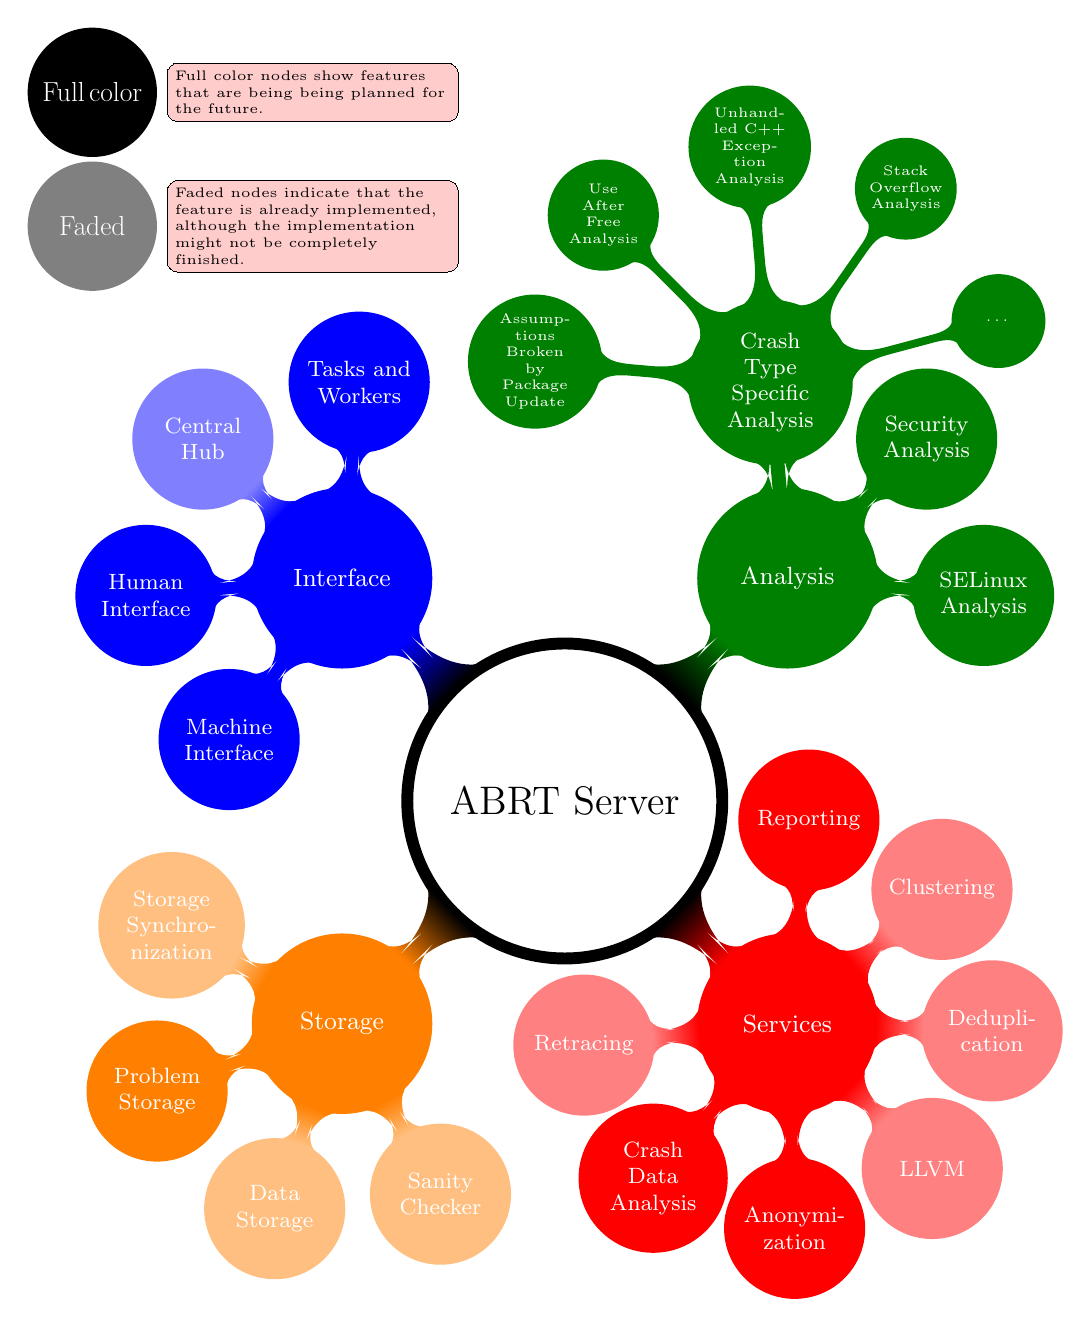
\begin{tikzpicture}[mindmap,
  every node/.style={concept},
  every annotation/.style={fill=red!20, line width=0, text=black},
  root concept/.append style={concept color=black, fill=white, line width=1ex, text=black, font=\Large},
  text=white,
  storage/.style={concept color=orange, faded/.style={concept color=orange!50}},
  services/.style={concept color=red, faded/.style={concept color=red!50}},
  interface/.style={concept color=blue, faded/.style={concept color=blue!50}},
  analysis/.style={concept color=green!50!black, faded/.style={concept color=green!25!black}},
  grow cyclic,
  level 1/.append style={level distance=4cm, sibling angle=90},
  level 2/.append style={level distance=2.5cm, sibling angle=50},
  level 3/.append style={level distance=3cm, sibling angle=40}]

  \node[concept color=black, scale=0.4, inner sep=0pt, outer sep=0pt] (planned) at (-6,9) {\Huge Full color};
  \node[annotation,right] at (planned.east) {Full color nodes show
    features that are being being planned for the future.};

  \node[concept color=black!50, scale=0.4, inner sep=0, outer sep=0pt] (implemented) at (-6,7.3) {\Huge Faded};
  \node[annotation,right] at (implemented.east) {Faded nodes indicate
    that the feature is already implemented, although the
    implementation might not be completely finished.};

  \node[root concept] {ABRT Server}
    child[storage] {node {Storage}
      child[faded] {node {Storage Synchronization}}
      child {node {Problem Storage}}
      child[faded] {node {Data Storage}}
      child[faded] {node {Sanity Checker}}
    }
    child[services] {node {Services}
      child[faded, sibling angle=43, level distance=2.6cm] {node {Retracing}}
      child[sibling angle=43, level distance=2.6cm] {node {Crash Data Analysis}}
      child[sibling angle=43, level distance=2.6cm] {node {Anonymi\-zation}}
      child[faded, sibling angle=43, level distance=2.6cm] {node {LLVM}}
      child[faded, sibling angle=43, level distance=2.6cm] {node {Dedupli\-cation}}
      child[faded, sibling angle=43, level distance=2.6cm] {node {Clustering}}
      child[sibling angle=43, level distance=2.6cm] {node {Reporting}}
    }
    child[analysis] {node {Analysis}
      child {node {SELinux Analysis}}
      child {node {Security Analysis}}
      child {node {Crash Type Specific Analysis}
        child {node {\ldots}}
        child {node {Stack Overflow Analysis}}
        child {node {Unhand\-led C++ Exception Analysis}}
        child {node {Use After Free Analysis}}
        child {node {Assump\-tions Broken by Package Update}}
      }
    }
    child[interface] {node {Interface}[clockwise from=100]
      child {node {Machine Interface}}
      child {node {Human Interface}}
      child[faded] {node {Central Hub}}
      child {node {Tasks and Workers}}
    };
\end{tikzpicture}
\end{center}

\begin{description}
\item[Storage] Server's storage is a combination of a database and a
  file server.
  \begin{description}
  \item[Storage Synchronization] Fetches data from external systems,
    such as RPMs and builds from Koji, bugs, comments, attachments
    from Red Hat Bugzilla, components, maintainers, releases from
    Fedora Package Database.
  \item[Problem Storage] We store all issues reported by users
    here. Problems can be program crashes, uncaught Python exceptions,
    Kernel oopses, VM cores, and SELinux denials.
  \item[Data Storage] We download and store RPMs of all versions of
    all packages in operating system.  This is necessary for correct
    retracing of both coredumps and minidumps.  We require both
    binaries and debugging information.  Static analysis requires data
    files from RPMs for greater accuracy.
  \item[Sanity Checker] We measure quality of data (builds, RPMs,
    bugs) downloaded from Fedora Project.  We found quality
    measurement and defect detection to be necessary to keep any
    service operational.  For example, many packages in Fedora and
    RHEL lacked proper debugging information, and this issue blocked
    retracing of many coredumps.  We started to track the quality of
    debugging information and watch for regressions.
  \end{description}
\item[Services] Separate services working on the top of Problem Storage
  and Data Storage. They are triggered by creating a new issue,
  changing the state of the issue, or at a certain time interval.
  \begin{description}
  \item[Retracing] Generates full backtrace from a coredump stored in
    Problem Storage. Generates function names from a minidump
    (coredump-level backtrace) stored in Problem Storage.
  \item[Crash Data Analysis] Depends on Retracing.
  \item[Anonymization] Depends on Crash Data Analysis.
  \item[LLVM] Depends on Anonymization.
  \item[Deduplication] Deduplication happens on several levels:
    minidumps (coredump-level backtraces) are compared when receiving
    a new issue.  Backtraces and/or function names (we call the list
    of function names from the crash thread \textit{optimized
      backtrace} in Faf) are compared when Retracing step is done.
    Analyzed issues are compared when the Crash Type Specific Analysis
    is done.
  \item[Clustering] Clustering finds clusters of issues that are close
    (similar) to each other. Clusters are created fro multiple
    distances. They are used to determine possible components and even
    program functions that are the root cause of the bug.
  \item[Reporting]
  \end{description}
\item[Analysis] Based on static analysis techniques applied to LLVM
  bitcode, the Analysis framework investigates reported issues and
  provide insight at the source code level.
  \begin{description}
  \item[Crash Type Specific Analysis]
  \item[Security Analysis]
  \item[SELinux Analysis]
  \end{description}
\item[Interface] World-facing communication is implemented in the
  web-based Human Interface, and JSON-based Machine Interface.
  Internal interactions between server parts are organized as tasks
  performed by workers. Task queue is managed by central hub, which
  also provides the public communication interfaces.
  \begin{description}
  \item[Human Interface]
  \item[Machine Interface]
  \item[Central Hub]
  \item[Tasks and Workers]
  \end{description}
\end{description}

\subsection{ABRT Server Services Overview}
\begin{center}
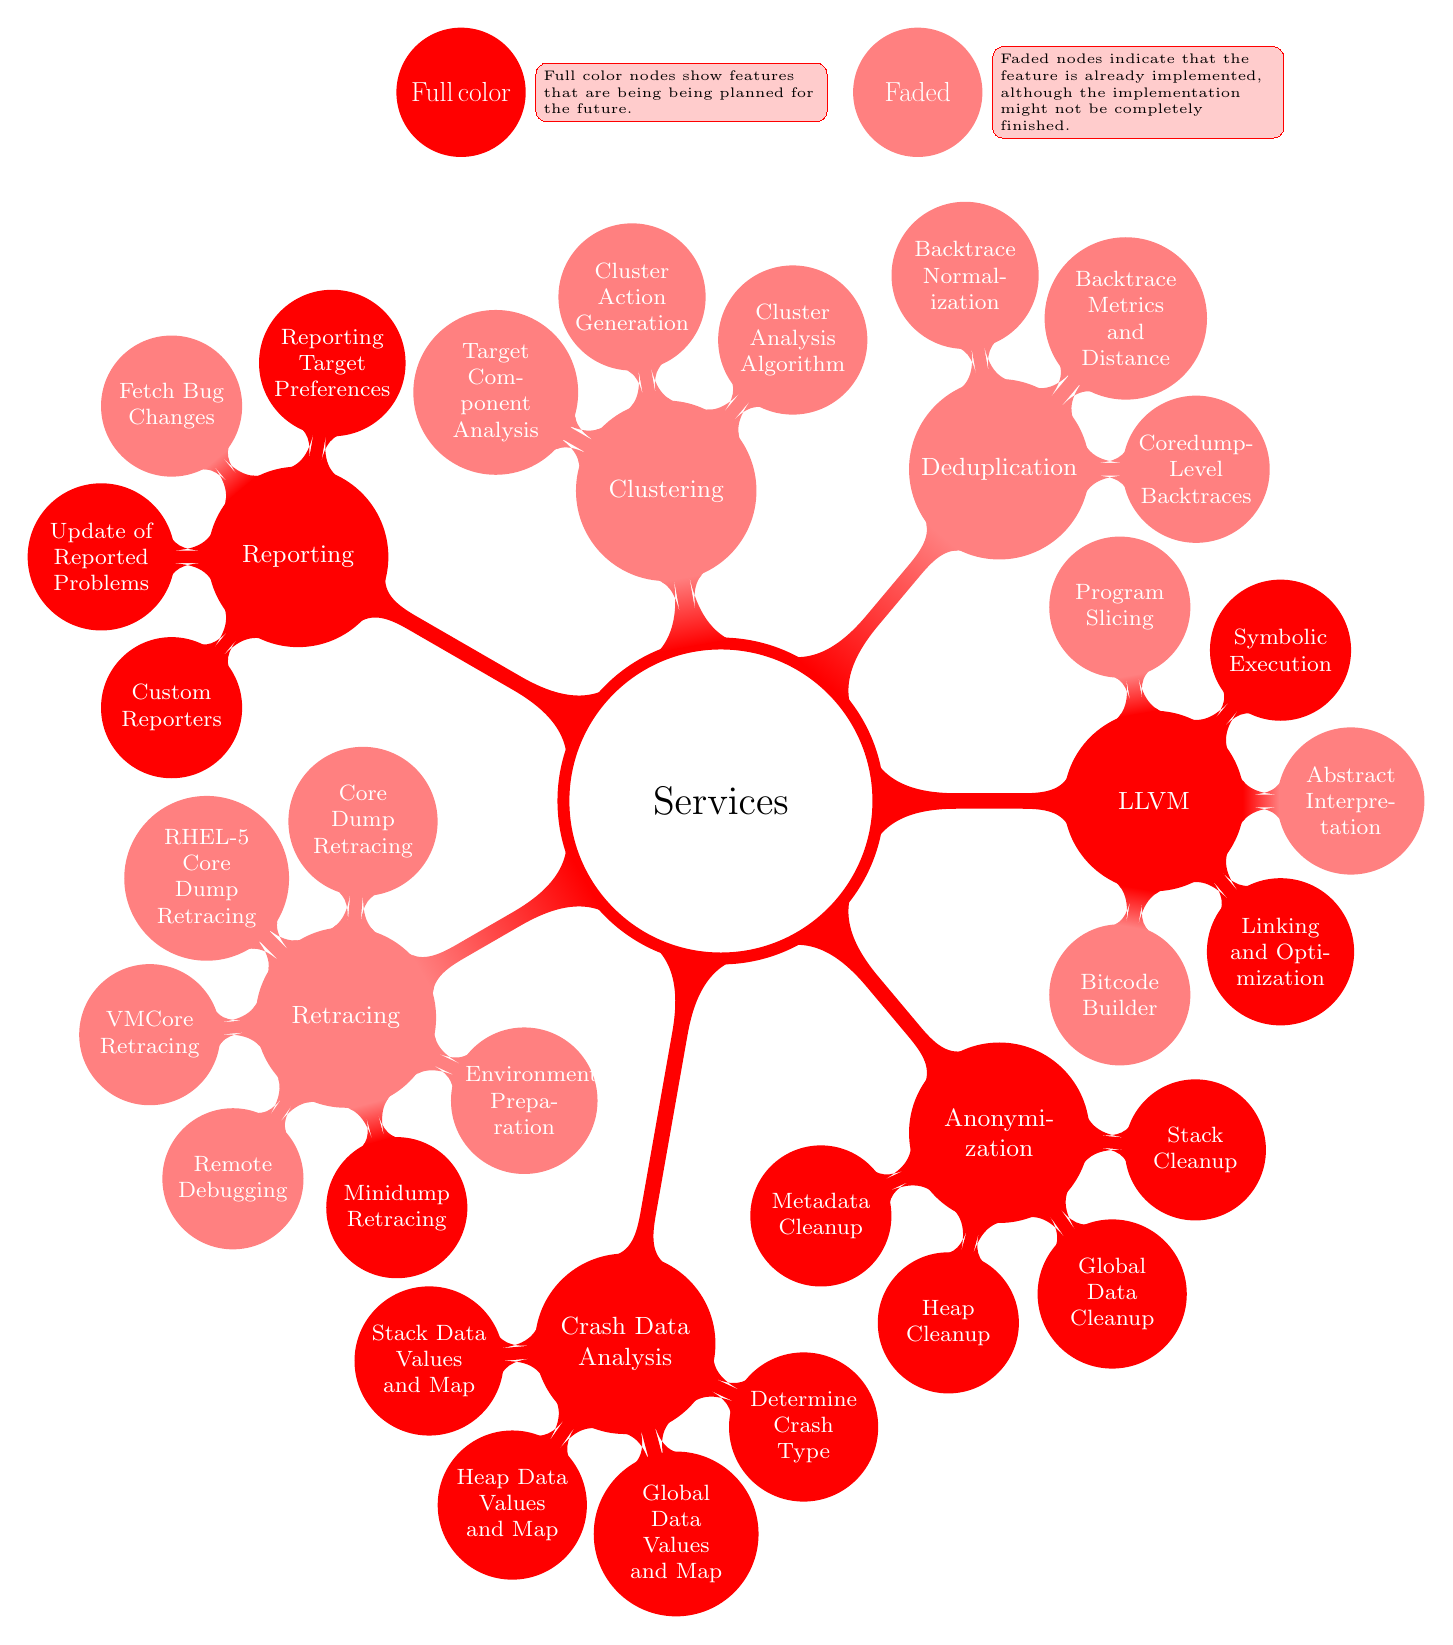
\begin{tikzpicture}[mindmap,
  every node/.style={concept, concept color=red},
  every annotation/.style={fill=red!20, line width=0, text=black},
  faded/.style={concept color=red!50},
  concept color=red,
  root concept/.append style={fill=white, line width=1ex, text=black, font=\Large},
  text=white,
  grow cyclic,
  level 1/.append style={level distance=5.5cm, sibling angle=50},
  level 2/.append style={level distance=2.5cm, sibling angle=50},
  level 3/.append style={level distance=3cm, sibling angle=40}]

  \node[scale=0.4, inner sep=0pt, outer sep=0pt] (planned) at (-3.3,9) {\Huge Full color};
  \node[annotation,right] at (planned.east) {Full color nodes show
    features that are being being planned for the future.};

  \node[faded, scale=0.4, inner sep=0, outer sep=0pt] (implemented) at (2.5,9) {\Huge Faded};
  \node[annotation,right] at (implemented.east) {Faded nodes indicate
    that the feature is already implemented, although the
    implementation might not be completely finished.};

  \node[root concept] {Services}
    child[faded] {node[faded] {Retracing}
      child[faded] {node[faded] {Core Dump Retracing}}
      child[faded] {node[faded] {RHEL-5 Core Dump Retracing}}
      child[faded] {node[faded] {VMCore Retracing}}
      child[faded] {node[faded] {Remote Debugging}}
      child[concept color=red] {node {Minidump Retracing}}
      child[faded] {node[faded] {Environment Preparation}}
    }
    child[level distance=7cm] {node {Crash Data Analysis}
      child {node {Stack Data Values and Map}}
      child {node {Heap Data Values and Map}}
      child {node {Global Data Values and Map}}
      child {node {Determine Crash Type}}
    }
    child {node {Anonymi\-zation}[clockwise from=45]
      child {node {Stack Cleanup}}
      child {node {Global Data Cleanup}}
      child {node {Heap Cleanup}}
      child {node {Metadata Cleanup}}
    }
    child {node {LLVM}
      child[faded] {node[faded] {Bitcode Builder}}
      child {node {Linking and Optimization}}
      child[faded] {node[faded] {Abstract Interpretation}}
      child {node {Symbolic Execution}}
      child[faded] {node[faded] {Program Slicing}}
    }
    child[faded] {node[faded] {Dedupli\-cation}
      child {node[faded] {Coredump-Level Backtraces}}
      child {node[faded] {Backtrace Metrics and Distance}}
      child {node[faded] {Backtrace Normalization}}
    }
    child[faded,level distance=4cm] {node[faded] {Clustering}
      child[faded] {node[faded] {Cluster Analysis Algorithm}}
      child[faded] {node[faded] {Cluster Action Generation}}
      child[faded] {node[faded] {Target Component Analysis}}
    }
    child[level distance=6.2cm] {node {Reporting}[clockwise from=80]
      child {node {Custom Reporters}}
      child {node {Update of Reported Problems}}
      child[faded] {node[faded] {Fetch Bug Changes}}
      child {node {Reporting Target Preferences}}
    };
\end{tikzpicture}
\end{center}

\subsection{ABRT Server Storage Overview}
\begin{center}
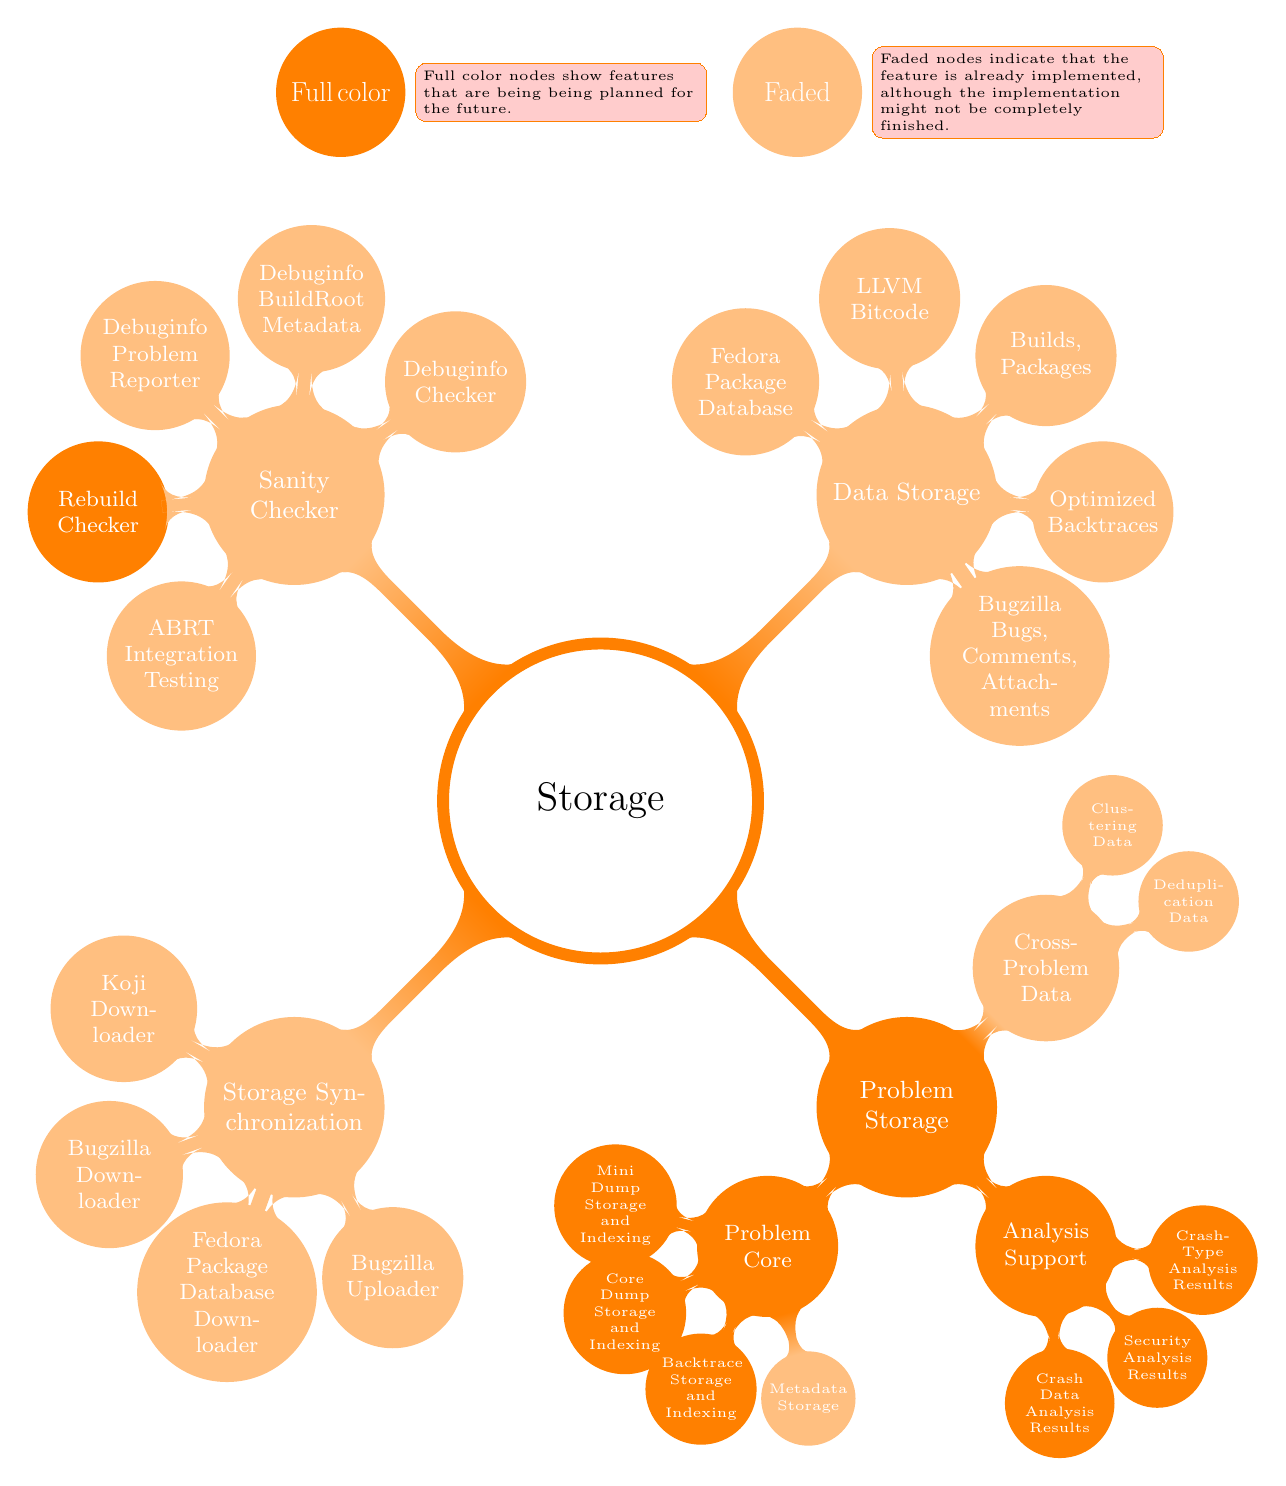
\begin{tikzpicture}[mindmap,
  every node/.style={concept, concept color=orange},
  every annotation/.style={fill=red!20, line width=0, text=black},
  faded/.style={concept color=orange!50},
  concept color=orange,
  root concept/.append style={fill=white, line width=1ex, text=black, font=\Large},
  text=white,
  grow cyclic,
  level 1/.append style={level distance=5.5cm, sibling angle=90},
  level 2/.append style={level distance=2.5cm, sibling angle=50},
  level 3/.append style={level distance=2cm, sibling angle=40}]

  \node[scale=0.4, inner sep=0pt, outer sep=0pt] (planned) at (-3.3,9) {\Huge Full color};
  \node[annotation,right] at (planned.east) {Full color nodes show
    features that are being being planned for the future.};

  \node[faded, scale=0.4, inner sep=0, outer sep=0pt] (implemented) at (2.5,9) {\Huge Faded};
  \node[annotation,right] at (implemented.east) {Faded nodes indicate
    that the feature is already implemented, although the
    implementation might not be completely finished.};

  \node[root concept] {Storage}
    child[faded] {node[faded] {Storage Synchronization}
      child {node[faded] {Koji Downloader}}
      child {node[faded] {Bugzilla Downloader}}
      child {node[faded] {Fedora Package Database Downloader}}
      child {node[faded] {Bugzilla Uploader}}
    }
    child {node {Problem Storage}
      child[sibling angle=90] {node {Problem Core}
        child {node {Mini Dump Storage and Indexing}}
        child {node {Core Dump Storage and Indexing}}
        child {node {Backtrace Storage and Indexing}}
        child[faded] {node[faded] {Metadata Storage}}
      }
      child[sibling angle=90] {node {Analysis Support}
        child {node {Crash Data Analysis Results}}
        child {node {Security Analysis Results}}
        child {node {Crash-Type Analysis Results}}
      }
      child[faded, sibling angle=90] {node[faded] {Cross-Problem Data}
        child[faded] {node[faded] {Dedupli\-cation Data}}
        child[faded] {node[faded] {Clus\-te\-ring Data}}
      }
    }
    child[faded] {node[faded] {Data Storage}
      child {node[faded] {Bugzilla Bugs, Comments, Attachments}}
      child {node[faded] {Optimized Backtraces}}
      child {node[faded] {Builds, Packages}}
      child {node[faded] {LLVM Bitcode}}
      child {node[faded] {Fedora Package Database}}
    }
    child[faded] {node[faded] {Sanity Checker}
      child[faded] {node[faded] {Debuginfo Checker}}
      child[faded] {node[faded] {Debuginfo BuildRoot Metadata}}
      child[faded] {node[faded] {Debuginfo Problem Reporter}}
      child {node {Rebuild Checker}}
      child[faded] {node[faded] {ABRT Integration Testing}}
    };
\end{tikzpicture}
\end{center}

\begin{description}
\item[Storage Synchronization]
  \begin{description}
  \item[Bugzilla Downloader] Downloads server-related bug reports from
    Red Hat Bugzilla.
  \end{description}
\item[Data Storage] Database and file storage for data required for
  the analysis, evaluation, and processing of reports and problems.
  \begin{description}
  \item[LLVM bitcode] We store LLVM bitcode of every binary and
    dynamic library compiled from C/C++ source code.
  \end{description}
\end{description}

\subsubsection{Problem Storage}
\begin{center}
\begin{tikzpicture}
\umlclass[x=-4,y=0]{problem}{
id : PRIMARY KEY \\
first occurrence : TIMESTAMP NOT NULL \\
last occurrence : TIMESTAMP NOT NULL \\
}{}

\umlclass[x=4,y=-2]{problem report}{
problem id : FOREIGN KEY NOT NULL \\
report id : FOREIGN KEY NOT NULL
}{}

\umlclass[x=4,y=2]{problem component}{
problem id : FOREIGN KEY NOT NULL \\
component id : FOREIGN KEY NOT NULL \\
order : INT NOT NULL
}{}

\umluniaggreg[geometry=|-,pos1=0.2,mult1=1,mult2=+,pos2=1.8]{problem}{problem report}
\umluniaggreg[geometry=|-,pos1=0.2,mult1=1,mult2=+,pos2=1.8]{problem}{problem component}

\end{tikzpicture}
\end{center}

Problems are dynamically created from reports.

\vfill
\subsubsection{Problem Storage -- Reports}

Part of reports is populated from $\mu$reports.

\begin{center}
\scalebox{0.9}{%
\begin{tikzpicture}
\umlclass[x=-4,y=0]{report}{
id : PRIMARY KEY AUTOINCREMENT \\
type : ENUM (USERSPACE, KERNEL, PYTHON, SELINUX) \\
first occurrence : TIMESTAMP \\
last occurrence : TIMESTAMP \\
count : INT \\
component id : FOREIGN KEY \\
problem id : FOREIGN KEY
}{}

\umlclass[x=-4,y=8]{report uptime}{
report id : FOREIGN KEY NOT NULL \\
uptime exp : INT NOT NULL \\
count : INT NOT NULL
}{}

\umlclass[x=5,y=6]{report executable}{
report id : FOREIGN KEY NOT NULL \\
path : STRING[512] NOT NULL \\
count : INT NOT NULL
}{}

\umlclass[x=5,y=3.4]{report arch}{
report id : FOREIGN KEY NOT NULL \\
arch id : FOREIGN KEY NOT NULL \\
count : INT NOT NULL
}{}

\umlclass[x=6,y=0]{report os release}{
report id : FOREIGN KEY NOT NULL \\
opsys release id : FOREIGN KEY NOT NULL \\
count : INT NOT NULL
}{}

\umlclass[x=6,y=-6.5]{report proc status}{
\begin{tabular}{l l}
id : PRIMARY KEY & capabilities bnd \\
report id : FOREIGN KEY & cpus allowed \\
traced : BOOL & mems allowed \\
utrace : INT & max cpu time \\
fd size : INT & max file size \\
vm peak : INT & max data size \\
vm size : INT & max stack size \\
vm data : INT & max core file size \\
vm stack : INT & max resident set \\
vm exe : INT & max processes \\

vm lib : INT & max open files \\
vm swap : INT & max locked memory \\
threads : INT & max address space \\
signal queue : INT & max file locks \\
signal pending & max pending signals \\
signal block & max msgqueue size \\
signal ignore & max nice priority \\
capabilities inherited & max realtime priority\\
capabilities prm & max realtime timeout \\
capabilities effective & \\
\end{tabular}
}{}

\umlclass[x=-4,y=-9]{report reason}{
report id : FOREIGN KEY NOT NULL \\
reason : STRING[512] NOT NULL \\
count : INT NOT NULL
}

\umluniaggreg[geometry=|-,pos1=0.2,mult1=1,mult2=+,pos2=1.9]{report}{report executable}
\umluniaggreg[geometry=|-,                 mult2=+,pos2=1.9]{report}{report arch}
\umluniaggreg[geometry=--,                 mult2=+,pos2=0.9]{report}{report uptime}
\umluniaggreg[geometry=--,mult1=1,pos1=0.15,mult2=+,pos2=0.85]{report}{report os release}
\umluniaggreg[geometry=|-,mult1=1,mult2=+,pos2=1.9]{report}{report proc status}
\umluniaggreg[geometry=--,                 mult2=+,pos2=0.9]{report}{report reason}

% Below report left
\end{tikzpicture}}
\end{center}

\subsubsection{Problem Storage -- Report backtraces}
\begin{center}
\begin{tikzpicture}
\umlclass[x=-4,y=0]{report}{}{}

\umlclass[x=4,y=3]{report bt hash}{
backtrace id : FOREIGN KEY NOT NULL \\
type : ENUM (NAMES, HASHES) NOT NULL \\
hash : STRING[64] NOT NULL \\
}{}

\umlclass[x=4,y=0]{report backtrace}{
id : PRIMARY KEY AUTOINCREMENT \\
report id : FOREIGN KEY
}{}

\umlclass[x=4,y=-3]{report bt frame}{
backtrace id : FOREIGN KEY \\
order : INT \\
symbol source id : FOREIGN KEY
}{}

\umluniaggreg[geometry=--,mult2=+,pos2=1.9]{report}{report backtrace}
\umluniaggreg[geometry=--,mult1=1,mult2=+]{report backtrace}{report bt frame}
\umluniaggreg[geometry=--,mult1=1,mult2=+]{report backtrace}{report bt hash}
\end{tikzpicture}
\end{center}


\subsubsection{Problem Storage -- Report packages}
\begin{center}
\begin{tikzpicture}
\umlclass[x=-4,y=0]{report}{}{}

\umlclass[x=4,y=2.6]{report package}{
id : PRIMARY KEY \\
report id : FOREIGN KEY NOT NULL \\
type : ENUM(CRASHED, RELATED) NOT NULL \\
installed package id : FOREIGN KEY NOT NULL \\
running package id : FOREIGN KEY \\
count : INT NOT NULL
}{}

\umlclass[x=4,y=-2.6]{report unknown package}{
id : PRIMARY KEY \\
report id : FOREIGN KEY NOT NULL \\
type : ENUM(CRASHED, RELATED) NOT NULL \\
name : STRING[64] NOT NULL \\
installed epoch : INT NOT NULL \\
installed version : STRING[64] NOT NULL \\
installed release : STRING[64] NOT NULL \\
installed arch id : FOREIGN KEY NOT NULL \\
running epoch : INT \\
running version : STRING[64] \\
running release : STRING[64] \\
running arch id : FOREIGN KEY \\
count : INT NOT NULL
}{}

\umluniaggreg[geometry=|-,pos1=0.2,mult1=1,mult2=+,pos2=1.9]{report}{report package}
\umluniaggreg[geometry=|-,pos1=0.2,mult1=1,mult2=+,pos2=1.9]{report}{report unknown package}
\end{tikzpicture}
\end{center}


\subsubsection{Problem Storage -- Report security aspects}
\begin{center}
\begin{tikzpicture}
\umlclass[x=-4,y=0]{report}{}{}

\umlclass[x=4,y=-1.5]{report selinux mode}{
report id : FOREIGN KEY NOT NULL \\
selinux mode : ENUM(DISABLED, PERMISSIVE, ENFORCING) NOT NULL \\
count : INT NOT NULL
}{}

\umlclass[x=1.2,y=1.5]{report selinux context}{
report id : FOREIGN KEY NOT NULL \\
context : STRING[256] NOT NULL \\
count : INT NOT NULL
}{}

\umluniaggreg[geometry=|-,pos1=0.2,mult1=1,mult2=+,pos2=1.9]{report}{report selinux mode}
\umluniaggreg[geometry=|-,pos1=0.2,mult1=1,mult2=+,pos2=1.9]{report}{report selinux context}
\end{tikzpicture}
\end{center}

\subsubsection{Problem Storage -- Report in-depth information}
Part of reports is populated from full reports.

\begin{center}
\begin{tikzpicture}
\umlclass[x=-4,y=0]{report}{}{}

\umlclass[x=2,y=-2]{report full backtrace}{
id : PRIMARY KEY \\
report id : FOREIGN KEY NOT NULL \\
os release id : FOREIGN KEY NOT NULL \\
text : STRING NOT NULL
}{}

\umlclass[x=2,y=2]{report coredump}{
id : PRIMARY KEY \\
report id : FOREIGN KEY NOT NULL \\
os release id : FOREIGN KEY NOT NULL
}{}

\umluniaggreg[geometry=|-,mult2=+,pos2=1.9]{report}{report full backtrace}
\umluniaggreg[geometry=|-,mult2=+,pos2=1.9]{report}{report coredump}

\end{tikzpicture}
\end{center}


\subsubsection{Problem Storage -- Report history}
\begin{center}
\begin{tikzpicture}
\umlclass[x=-4,y=0]{report}{}{}

\umlclass[x=5,y=-3]{report history daily}{
day : DATE NOT NULL \\
opsys release id : FOREIGN KEY NOT NULL \\
report id : FOREIGN KEY NOT NULL \\
count : INT NOT NULL
}{}

\umlclass[x=5,y=0]{report history weekly}{
week : DATE NOT NULL\\
opsys release id : FOREIGN KEY NOT NULL \\
report id : FOREIGN KEY NOT NULL \\
count : INT NOT NULL
}{}

\umlclass[x=5,y=3]{report history monthly}{
report id : FOREIGN KEY NOT NULL \\
opsys release id : FOREIGN KEY NOT NULL \\
month : DATE NOT NULL \\
count : INT NOT NULL
}{}

\umluniaggreg[geometry=-|-,pos1=0.2,mult1=1,mult2=*,pos2=1.8]{report}{report history daily}
\umluniaggreg[geometry=--,pos1=0.2,mult2=*,pos2=0.9]{report}{report history weekly}
\umluniaggreg[geometry=-|-,pos1=0.2,mult2=*,pos2=1.8]{report}{report history monthly}

\end{tikzpicture}
\end{center}

\subsubsection{Problem Storage -- Symbols}
\begin{center}
\begin{tikzpicture}
\umlclass[x=-4,y=0]{symbol}{
id : PRIMARY KEY \\
name : STRING NOT NULL \\
normalized path : STRING NOT NULL
}{}

\umlclass[x=4,y=0]{symbol source}{
symbol id : FOREIGN KEY \\
build id : STRING NOT NULL \\
path : STRING NOT NULL \\
offset : INT NOT NULL \\
source file : STRING \\
hash : STRING \\
line number : INT
}{}

\umluniaggreg[geometry=--,pos1=0.2,mult1=1,mult2=+,pos2=0.8]{symbol}{symbol source}
\end{tikzpicture}
\end{center}

\subsubsection{Problem Storage -- Clusters}

\subsubsection{Data Storage -- Builds}
\begin{center}
\begin{tikzpicture}
\umlclass[x=-4,y=0]{opsys}{
id : PRIMARY KEY \\
name : STRING[32] NOT NULL
}

\umlclass[x=6,y=0]{opsys release}{
id : PRIMARY KEY \\
opsys id : FOREIGN KEY NOT NULL \\
version : STRING[32] \\
releasedate = DATETIME
}

\umlclass[x=-4,y=-5]{opsys component}{
id : PRIMARY KEY \\
name : STRING[64] NOT NULL \\
opsys id : FOREIGN KEY NOT NULL
}

\umlclass[x=6,y=-5]{build}{
id : PRIMARY KEY \\
secondary id : INT \\
component id : FOREIGN KEY NOT NULL \\
epoch : INT NOT NULL \\
version : STRING[64] NOT NULL \\
release : STRING[64] NOT NULL
}

\umlclass[x=-4,y=-10]{tag}{
id : PRIMARY KEY \\
opsys id : FOREIGN KEY \\
name : STRING[32] NOT NULL \\
perm : INT \\
locked : BOOL NOT NULL
}

\umlclass[x=6,y=-10]{tag inheritance}{
tag id : FOREIGN KEY NOT NULL \\
parent id : FOREIGN KEY NOT NULL \\
intransitive : BOOL NOT NULL \\
priority : INT NOT NULL \\
noconfig : INT NOT NULL
}

\umluniaggreg[geometry=--,pos1=0.2,mult1=1,mult2=*,pos2=0.8]{opsys}{opsys release}
\umlassoc[geometry=|-|,pos1=0.2,mult1=*,mult2=*,pos2=2.8]{opsys release}{opsys component}
\umluniaggreg[geometry=--,pos1=0.2,mult1=1,mult2=*,pos2=0.8]{opsys component}{build}
\umlassoc[geometry=|-|,pos1=0.2,mult1=*,mult2=*,pos2=2.8]{build}{tag}
\umluniassoc[geometry=--,pos1=0.2,mult1=1,mult2=*,pos2=0.8]{tag}{tag inheritance}
\end{tikzpicture}
\end{center}

\subsubsection{Data Storage -- Packages}
\begin{center}
\begin{tikzpicture}
\umlclass[x=0,y=4]{arch}{
id : PRIMARY KEY \\
name : STRING[8] NOT NULL
}

\umlclass[x=0,y=0]{package}{
id : PRIMARY KEY \\
secondary id : INT
build id : FOREIGN KEY NOT NULL \\
arch id : FOREIGN KEY NOT NULL \\
name : STRING[64] NOT NULL
}

\umlclass[x=0,y=-5]{package dependency}{
id : PRIMARY KEY \\
package id : FOREIGN KEY NOT NULL \\
type : ENUM(REQUIRES PROVIDES CONFLICTS OBSOLETES) NOT NULL \\
symbol : STRING[512] NOT NULL \\
flags : INT NOT NULL \\
epoch : INT \\
version : STRING[64] \\
release : STRING[64]
}

\umluniassoc[geometry=--,pos1=0.2,mult1=1,mult2=*,pos2=0.8]{package}{arch}
\umluniaggreg[geometry=--,pos1=0.2,mult1=1,mult2=*,pos2=0.8]{package}{package dependency}
\end{tikzpicture}
\end{center}

\subsubsection{Data Storage -- Red Hat Bugzilla}
\begin{center}
\begin{tikzpicture}
\umlclass[x=0,y=0]{rhbz bug}{
id : PRIMARY KEY \\
summary : STRING[256] NOT NULL \\
status : ENUM(CLOSED, ASSIGNED, NEW, MODIFIED, VERIFIED, \\
\hspace{5mm}ON QA, ON DEV, RELEASE PENDING, POST) NOT NULL \\
resolution : ENUM(NOTABUG, WONTFIX, WORKSFORME, \\
\hspace{5mm}DEFERRED, CURRENTRELEASE, RAWHIDE, ERRATA, \\
\hspace{5mm}DUPLICATE, UPSTREAM, NEXTRELEASE, CANTFIX, \\
\hspace{5mm}INSUFFICIENT DATA)
resolution dup id : FOREIGN KEY \\
created : DATE NOT NULL \\
last change : DATE NOT NULL \\
opsys release id : FOREIGN KEY NOT NULL \\
opsys component : FOREIGN KEY NOT NULL \\
whiteboard : STRING[512] \\
creator id : FOREIGN KEY NOT NULL
}

\umlclass[x=4.5,y=-9]{rhbz attachment}{
id : PRIMARY KEY \\
bug id : FOREIGN KEY NOT NULL \\
creator id : FOREIGN KEY NOT NULL \\
mime type : STRING[128] NOT NULL \\
description : STRING[256] \\
created : DATE NOT NULL \\
last changed : DATE NOT NULL \\
is private : BOOL NOT NULL \\
is patch : BOOL NOT NULL \\
is obsolete : BOOL NOT NULL \\
is url : BOOL NOT NULL \\
file name : STRING[512]
}

\umlclass[x=-4.5,y=-9.0]{rhbz comment}{
id : PRIMARY KEY \\
secondary id : INT NOT NULL \\
bug id : FOREIGN KEY NOT NULL \\
creator id : FOREIGN KEY NOT NULL \\
number : INT NOT NULL \\
is private : BOOL NOT NULL \\
body : STRING[2048] \\
created : DATE NOT NULL \\
type : ENUM(NORMAL, DUPE OF, HAS DUPE, \\
\hspace{5mm}MOVED TO, POPULAR VOTES, \\
\hspace{5mm}ATTACHMENT CREATED, ATTACHMENT UPDATED) \\
duplicate id : FOREIGN KEY \\
attachment id : FOREIGN KEY
}

\umluniaggreg[geometry=|-|,pos1=0.2,mult1=1,mult2=*,pos2=2.8]{rhbz bug}{rhbz attachment}
\umluniaggreg[geometry=|-|,pos1=0.2,mult1=1,mult2=+,pos2=2.8]{rhbz bug}{rhbz comment}

\end{tikzpicture}
\end{center}

\subsubsection{Data Storage -- Red Hat Bugzilla Users}
\begin{center}
\begin{tikzpicture}
\umlclass[x=-4,y=0]{RhbzUser}{
id : PRIMARY KEY \\
email : STRING[256] NOT NULL \\
can login : BOOL NOT NULL \\
name : STRING[256] NOT NULL \\
real name : STRING[256]
}

\umlclass[x=4,y=-2]{RhbzBug}{
}

\umlclass[x=4,y=0]{RhbzAttachment}{
}

\umlclass[x=4,y=2]{RhbzComment}{
}

\umluniassoc[geometry=-|-,pos1=0.2,mult1=*,mult2=1,pos2=2.8]{RhbzBug}{RhbzUser}
\umluniassoc[geometry=-|-,pos1=0.2,mult1=*,mult2=1,pos2=2.8]{RhbzComment}{RhbzUser}
\umluniassoc[geometry=--,pos1=0.2,mult1=*]{RhbzAttachment}{RhbzUser}
\end{tikzpicture}
\end{center}

\subsubsection{Data Storage -- LLVM Bitcode}
\begin{center}
\begin{tikzpicture}
\umlclass[x=-4,y=0]{LlvmBuild}{
id : PRIMARY KEY \\
build id : FOREIGN KEY NOT NULL \\
started : DATE NOT NULL \\
duration : INT NOT NULL \\
success : BOOL NOT NULL \\
arch id : FOREIGN KEY NOT NULL \\
llvm build id : FOREIGN KEY NOT NULL \\
build log
}

\umlclass[x=4,y=0]{LlvmBitcode}{
llvm build id : FOREIGN KEY NOT NULL \\
path : STRING[512] NOT NULL \\
}
% the following empty line is mandatory to avoid TeX stack overflow

\end{tikzpicture}
\end{center}

\subsubsection{Sanity Checker -- Debuginfo checker}
\begin{center}
\begin{tikzpicture}
\umlclass[x=4,y=-10.5]{DebuginfoMissingSymlink}{
build id : FOREIGN KEY NOT NULL \\
debuginfo symlink : STRING[512] NOT NULL \\
binary symlink : STRING[512] NOT NULL \\
debuginfo package id : FOREIGN KEY NOT NULL
}

\umlclass[x=4,y=-7.1]{DebuginfoSymlinkPointingToAnotherPath}{
build id : FOREIGN KEY NOT NULL \\
package id : FOREIGN KEY NOT NULL \\
debuginfo symlink path : STRING[512] NOT NULL \\
symlink target path : STRING[512] NOT NULL \\
symlink package id : FOREIGN KEY
}

\umlclass[x=4,y=-3.5]{DebuginfoMissingForBinary}{
build id : FOREIGN KEY NOT NULL \\
path : STRING[512] NOT NULL \\
package id : FOREIGN KEY NOT NULL \\
stripped : BOOLEAN \\
mode : INT
}

\umlclass[x=4,y=0]{DebuginfoUnused}{
build id : FOREIGN KEY NOT NULL \\
debuginfo path : STRING[512] NOT NULL \\
binary path : STRING[512] NOT NULL \\
size : INT NOT NULL
}

\umlclass[x=4,y=3]{DebuginfoMissingSourceFile}{
build id : FOREIGN KEY NOT NULL \\
debuginfo path : STRING[512] NOT NULL \\
source path : STRING[512] NOT NULL
}

\umlclass[x=4,y=6]{DebuginfoMissingSection}{
build id : FOREIGN KEY NOT NULL \\
path : STRING[512] NOT NULL \\
package id : FOREIGN KEY NOT NULL
}

\umlclass[x=-6,y=-2]{build}{
}

\umluniassoc[geometry=-|-,pos1=0.1,mult1=1,mult2=*,pos2=2.8]{build}{DebuginfoMissingSymlink}
\umluniassoc[geometry=-|-,                 mult2=*,pos2=2.8]{build}{DebuginfoSymlinkPointingToAnotherPath}
\umluniassoc[geometry=-|-,                 mult2=*,pos2=2.8]{build}{DebuginfoMissingForBinary}
\umluniassoc[geometry=-|-,                 mult2=*,pos2=2.8]{build}{DebuginfoUnused}
\umluniassoc[geometry=-|-,                 mult2=*,pos2=2.8]{build}{DebuginfoMissingSourceFile}
\umluniassoc[geometry=-|-,                 mult2=*,pos2=2.8]{build}{DebuginfoMissingSection}
% the following empty line is mandatory to avoid TeX stack overflow

\end{tikzpicture}
\end{center}

\begin{center}
\begin{tikzpicture}
\umlclass[x=4,y=-10]{DebuginfoInvalidVersion}{
build id : FOREIGN KEY NOT NULL \\
line table version : STRING[16] NOT NULL \\
line table offset : INT NOT NULL \\
compilation unit offset : INT NOT NULL \\
debuginfo path : STRING[512] NOT NULL \\
package id : FOREIGN KEY NOT NULL
}

\umlclass[x=4,y=-6]{DebuginfoRelativeSourceNameNoCompDir}{
build id : FOREIGN KEY NOT NULL \\
debuginfo path : STRING[512] NOT NULL \\
package id : FOREIGN KEY NOT NULL \\
compilation unit offset : INT NOT NULL \\
source path : STRING[512] NOT NULL
}

\umlclass[x=4,y=-2]{DebuginfoMissingCompDir}{
build id : FOREIGN KEY NOT NULL \\
debuginfo path : STRING[512] NOT NULL \\
compilation unit offset : INT NOT NULL \\
table offset : INT NOT NULL \\
source path : STRING[512] NOT NULL
}

\umlclass[x=4,y=2]{DebuginfoRelativeDirectory}{
build id : FOREIGN KEY NOT NULL \\
debuginfo path : STRING[512] NOT NULL \\
table offset : INT NOT NULL \\
directory offset : INT NOT NULL \\
directory name : STRING[512] NOT NULL \\
source path : STRING[512] NOT NULL \\
compilation unit offset : INT NOT NULL
}

\umlclass[x=4,y=6]{DebuginfoInvalidDirectoryOffset}{
build id : FOREIGN KEY NOT NULL \\
debuginfo path : STRING[512] NOT NULL \\
table offset : INT NOT NULL \\
directory offset : INT NOT NULL \\
source path : STRING[512] NOT NULL
}

\umlclass[x=-6,y=-2]{build}{
}

\umluniassoc[geometry=-|-,pos1=0.1,mult1=1,mult2=*,pos2=2.8]{build}{DebuginfoInvalidVersion}
\umluniassoc[geometry=-|-,                 mult2=*,pos2=2.8]{build}{DebuginfoRelativeSourceNameNoCompDir}
\umluniassoc[geometry=-|-,                 mult2=*,pos2=2.8]{build}{DebuginfoMissingCompDir}
\umluniassoc[geometry=-|-,                 mult2=*,pos2=2.8]{build}{DebuginfoRelativeDirectory}
\umluniassoc[geometry=-|-,                 mult2=*,pos2=2.8]{build}{DebuginfoInvalidDirectoryOffset}
% the following empty line is mandatory to avoid TeX stack overflow

\end{tikzpicture}
\end{center}

\begin{center}
\begin{tikzpicture}
\umlclass[x=4,y=-2]{DebuginfoSourceRebuild}{
build id : FOREIGN KEY NOT NULL \\
status : ENUM( \\
\hspace{5mm}INSTALL RPM DEPENDENCIES FAILED, \\
\hspace{5mm}PREPARE BUILD ENVIRONMENT FAILED, \\
\hspace{5mm}BUILD SRPM FAILED, \\
\hspace{5mm}DEBUGSOURCES NOT FOUND, \\
\hspace{5mm}CLEAN FAILED, \\
\hspace{5mm}SUCCESS)
}

\umlclass[x=4,y=2]{DebuginfoSourceFile}{
build id : FOREIGN KEY NOT NULL \\
source path : STRING[512] NOT NULL
}

\umlclass[x=-6,y=0]{build}{
}

\umluniassoc[geometry=-|-,pos1=0.1,mult1=1,mult2=*,pos2=2.8]{build}{DebuginfoSourceRebuild}
\umluniassoc[geometry=-|-,                 mult2=*,pos2=2.8]{build}{DebuginfoSourceFile}
% the following empty line is mandatory to avoid TeX stack overflow

\end{tikzpicture}
\end{center}

\subsection{ABRT Server Interface Overview}
\begin{center}
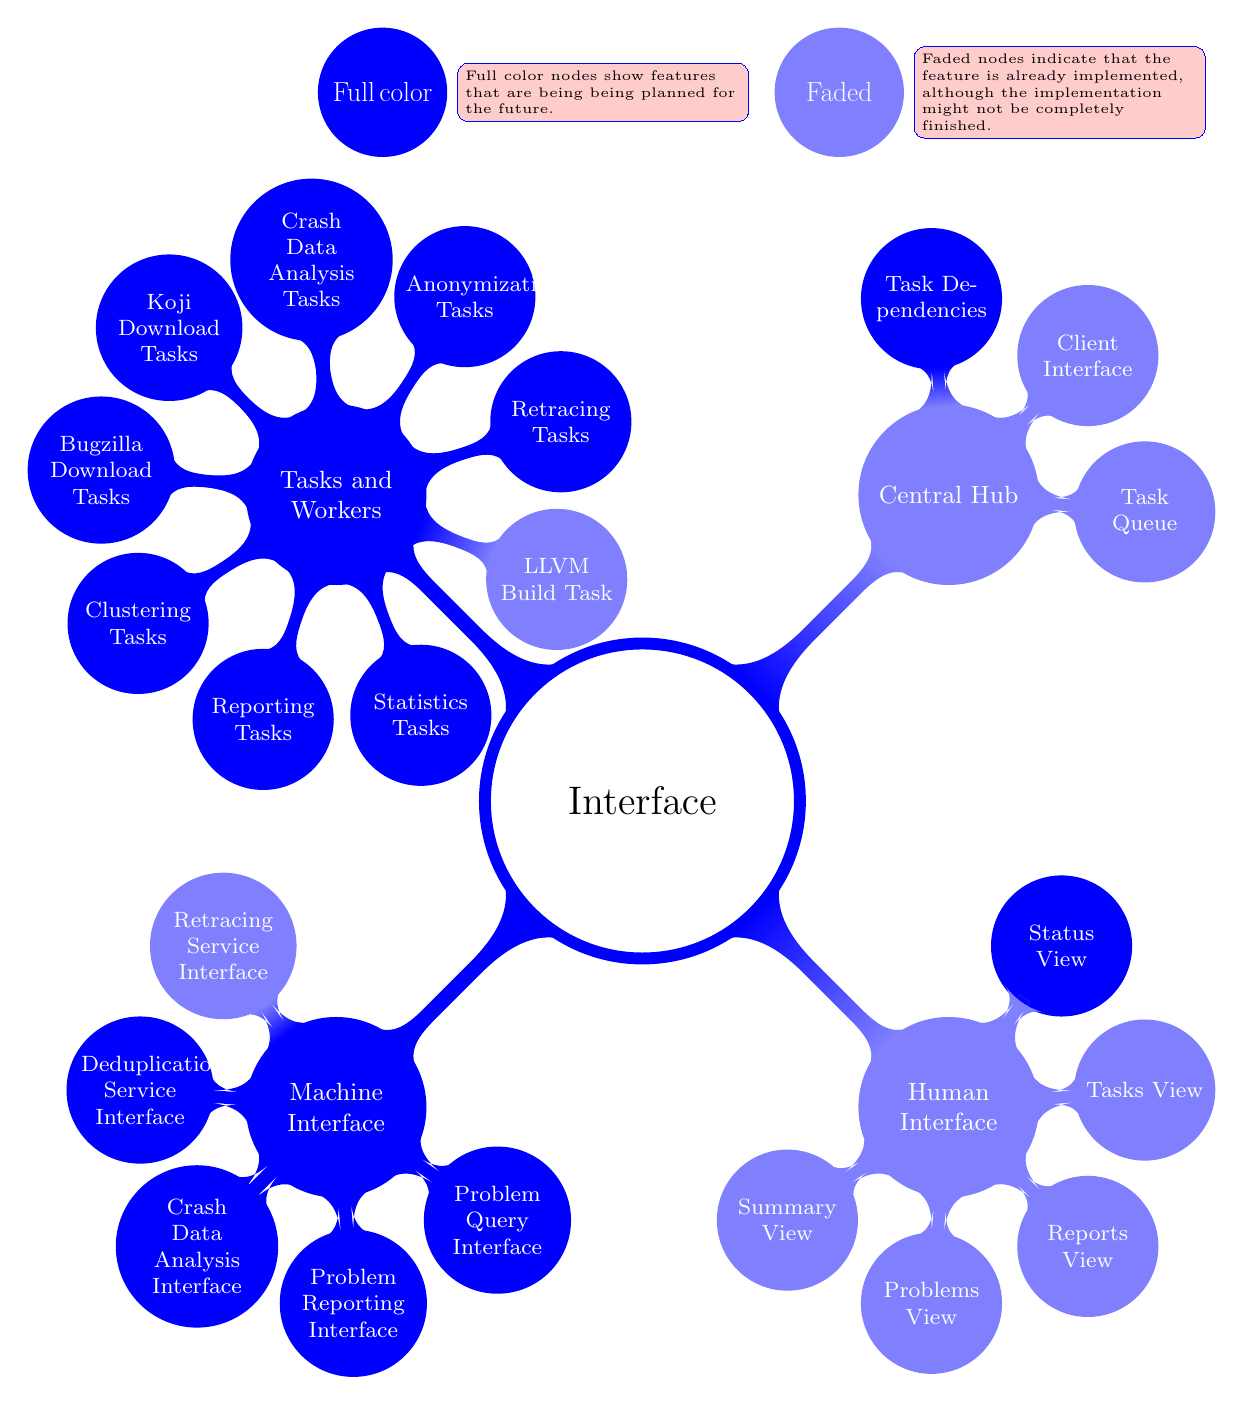
\begin{tikzpicture}[mindmap,
  every node/.style={concept, concept color=blue},
  every annotation/.style={fill=red!20, line width=0, text=black},
  faded/.style={concept color=blue!50},
  concept color=blue,
  root concept/.append style={fill=white, line width=1ex, text=black, font=\Large},
  text=white,
  grow cyclic,
  level 1/.append style={level distance=5.5cm, sibling angle=90},
  level 2/.append style={level distance=2.5cm, sibling angle=50},
  level 3/.append style={level distance=2cm, sibling angle=40}]

  \node[scale=0.4, inner sep=0pt, outer sep=0pt] (planned) at (-3.3,9) {\Huge Full color};
  \node[annotation,right] at (planned.east) {Full color nodes show
    features that are being being planned for the future.};

  \node[faded, scale=0.4, inner sep=0, outer sep=0pt] (implemented) at (2.5,9) {\Huge Faded};
  \node[annotation,right] at (implemented.east) {Faded nodes indicate
    that the feature is already implemented, although the
    implementation might not be completely finished.};

  \node[root concept] {Interface}
    child {node {Machine Interface}
      child[faded] {node[faded] {Retracing Service Interface}}
      child {node {Deduplication Service Interface}}
      child {node {Crash Data Analysis Interface}}
      child {node {Problem Reporting Interface}}
      child {node {Problem Query Interface}}
    }
    child[faded] {node[faded] {Human Interface}
      child[faded] {node[faded] {Summary View}}
      child[faded] {node[faded] {Problems View}}
      child[faded] {node[faded] {Reports View}}
      child[faded] {node[faded] {Tasks View}}
      child {node {Status View}}
    }
    child[faded] {node[faded] {Central Hub}
      child {node[faded] {Task Queue}}
      child {node[faded] {Client Interface}}
      child[concept color=blue] {node {Task Dependencies}}
    }
    child {node {Tasks and Workers}
      child[faded, sibling angle=39, level distance=3cm] {node[faded] {LLVM Build Task}}
      child[sibling angle=39, level distance=3cm] {node {Retracing Tasks}}
      child[sibling angle=39, level distance=3cm] {node {Anonymization Tasks}}
      child[sibling angle=39, level distance=3cm] {node {Crash Data Analysis Tasks}}
      child[sibling angle=39, level distance=3cm] {node {Koji Download Tasks}}
      child[sibling angle=39, level distance=3cm] {node {Bugzilla Download Tasks}}
      child[sibling angle=39, level distance=3cm] {node {Clustering Tasks}}
      child[sibling angle=39, level distance=3cm] {node {Reporting Tasks}}
      child[sibling angle=39, level distance=3cm] {node {Statistics Tasks}}
    };
\end{tikzpicture}
\end{center}

\subsubsection{Summary Page}

\begin{center}
\begin{tabular}{|c|c|c|c|}
\hline
HTTP Verb & Path & Format & Used for \\
\hline
\texttt{GET} & \texttt{/summary} & HTML & Display the report summary graph. \\
\hline
\end{tabular}
\end{center}


\begin{center}
\shadowbox{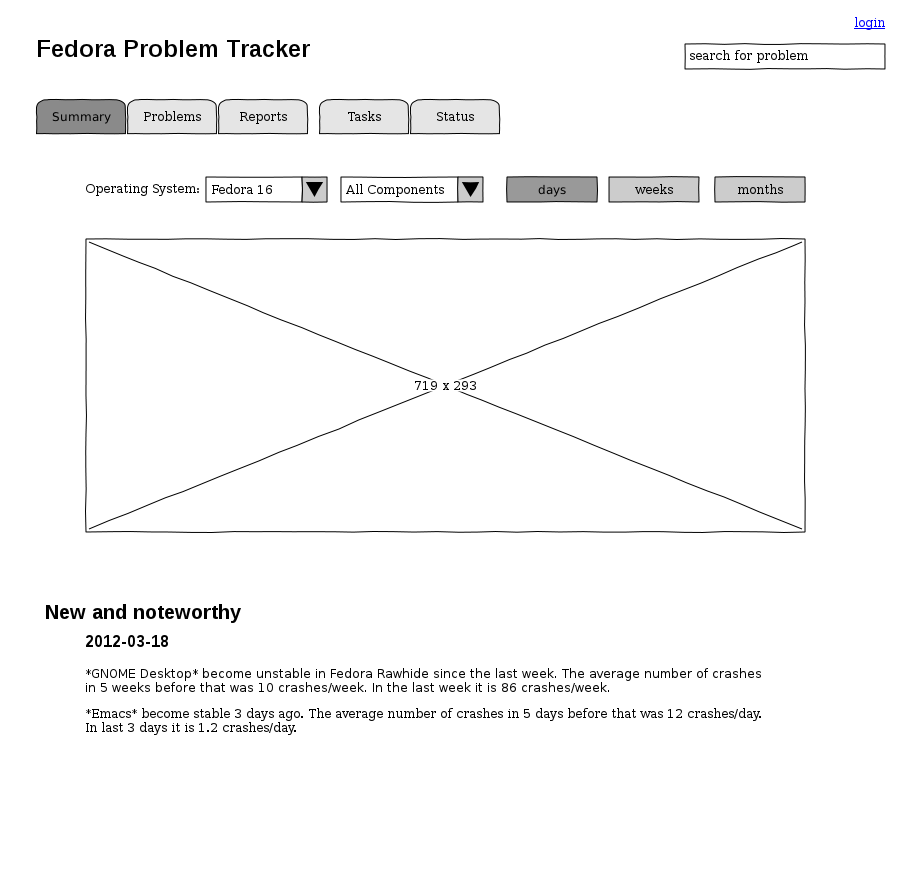
\includegraphics[width=\textwidth, trim=0 3cm 0 0, clip=true]{server-ui-summary.png}}
\end{center}

\begin{description}
\item[Operating System] The available options include Fedora releases,
  pre-release branched Fedora, Fedora Rawhide, All. The list of
  releases should be obtained from Fedora Package Database (this is
  handled by Storage Synchronization.
\item[Components] The available options include All Components, the
  list of all components for the selected Operating System, and
  selected \texttt{comps.xml} groups (such as GNOME Desktop, KDE
  Desktop, Xfce, Web Server, Electronic Lab, Engineering and
  Scientific, Font design and packaging, System Tools, Sound and
  Video, Office/Productivity)
\item[Graph] Displays the number of problems (individual events) in
  time. The underlying data are updated once a day.
\item[Days] The graph shows problems in the last 14 days.
\item[Weeks] The graph shows problems in the last 12 weeks (3 months).
\item[Months] The graph shows problems in the last 12 months.
\item[New and noteworthy] Shows automatically discovered interesting
  trends that can be detected from data.  It tells visitor which
  combinations of Operating System and Component might be worth
  looking.
\end{description}

\subsubsection{Problems Overview Page}

\begin{center}
\begin{tabular}{|c|c|c|c|}
\hline
HTTP Verb & Path & Format & Used for \\
\hline
\texttt{GET} & \texttt{/problems} & HTML & Display the report summary graph. \\
\hline
\end{tabular}
\end{center}

\begin{center}
\shadowbox{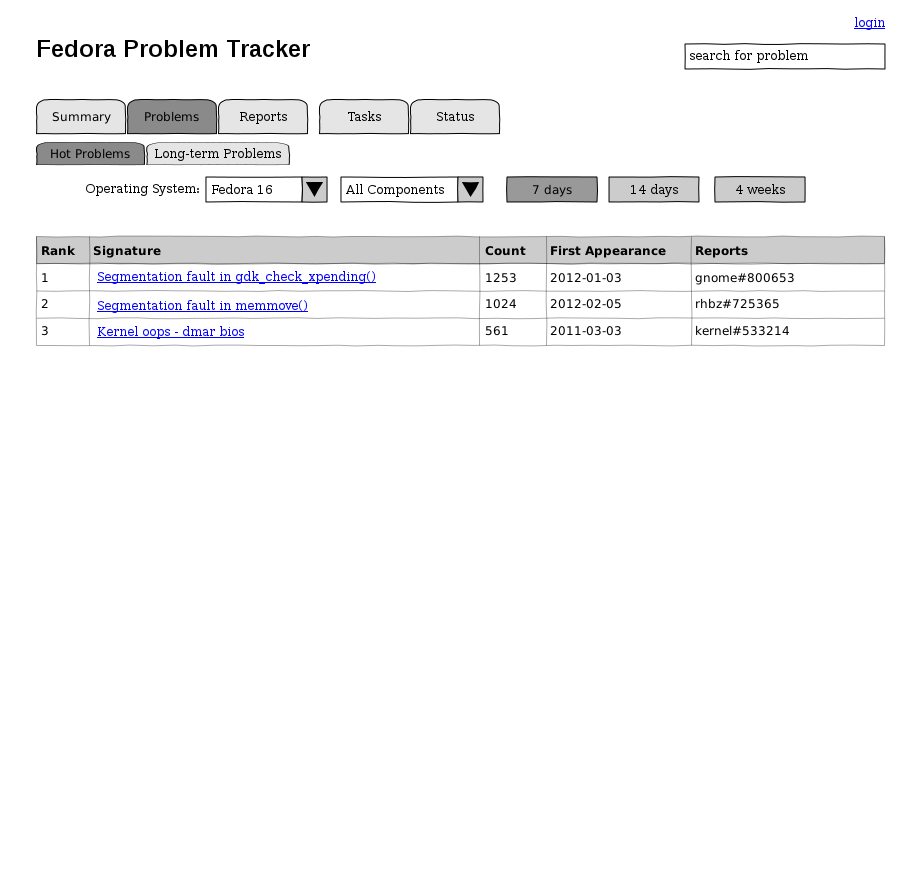
\includegraphics[width=\textwidth, trim=0 16cm 0 0, clip=true]{server-ui-problems-overview.png}}
\end{center}

\subsubsection{Problems Item Summary Page}
\begin{center}
\shadowbox{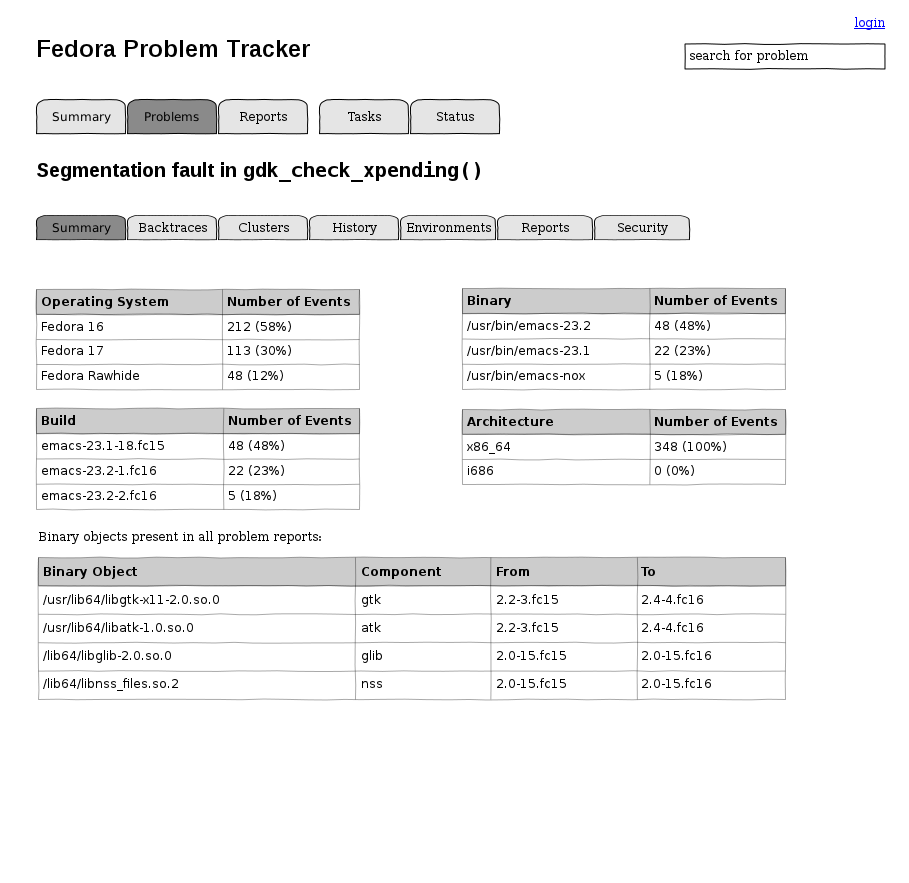
\includegraphics[width=\textwidth, trim=0 5cm 0 0, clip=true]{server-ui-problems-item-summary.png}}
\end{center}

\subsubsection{Reports Overview Page}
\begin{center}
\shadowbox{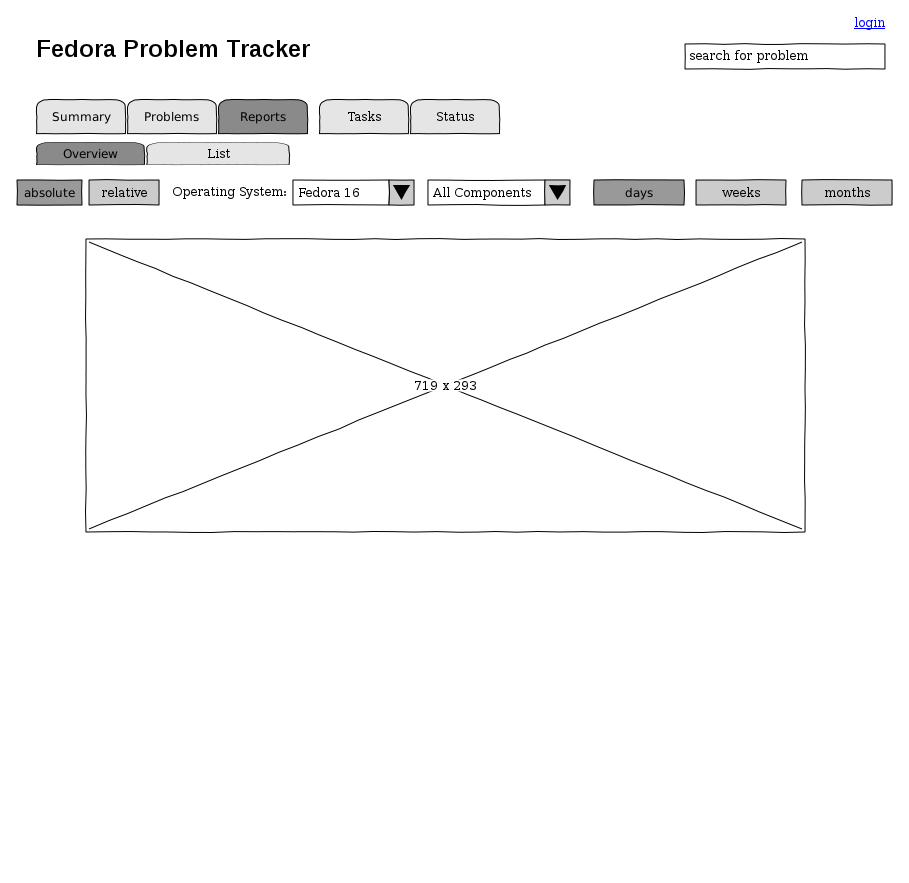
\includegraphics[width=\textwidth, trim=0 10cm 0 0, clip=true]{server-ui-reports-overview.png}}
\end{center}

\subsubsection{Reports List Page}
\begin{center}
\shadowbox{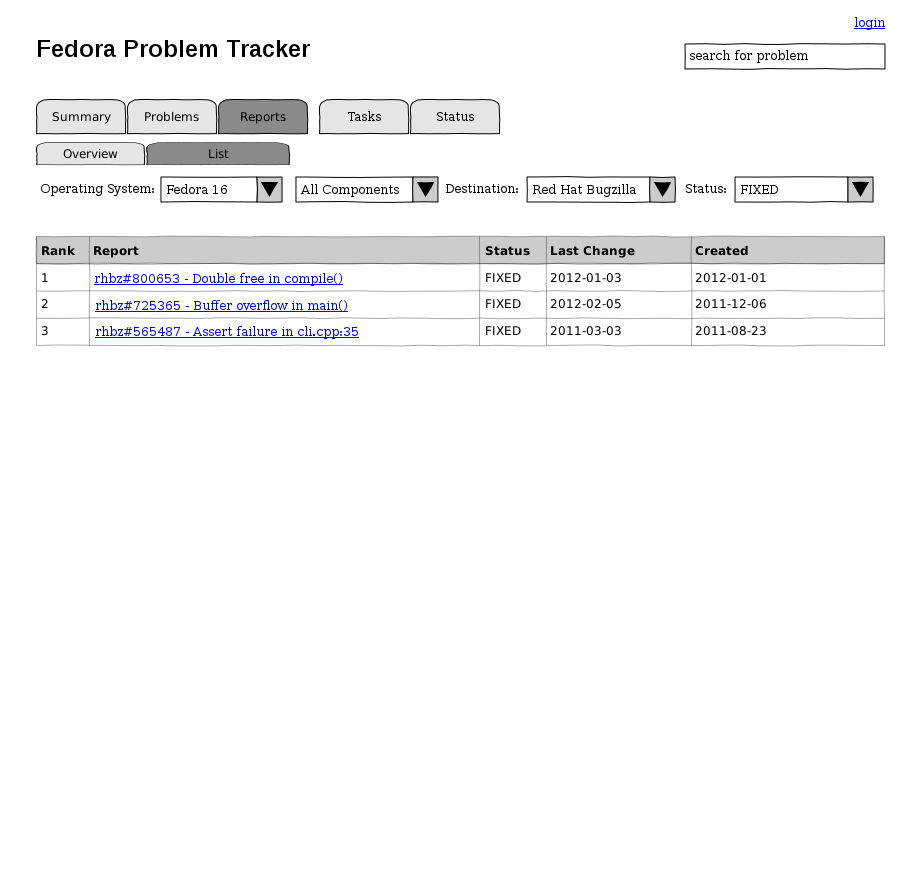
\includegraphics[width=\textwidth, trim=0 16cm 0 0, clip=true]{server-ui-reports-list.png}}
\end{center}

\subsubsection{Server Tasks Page}
\begin{center}
\shadowbox{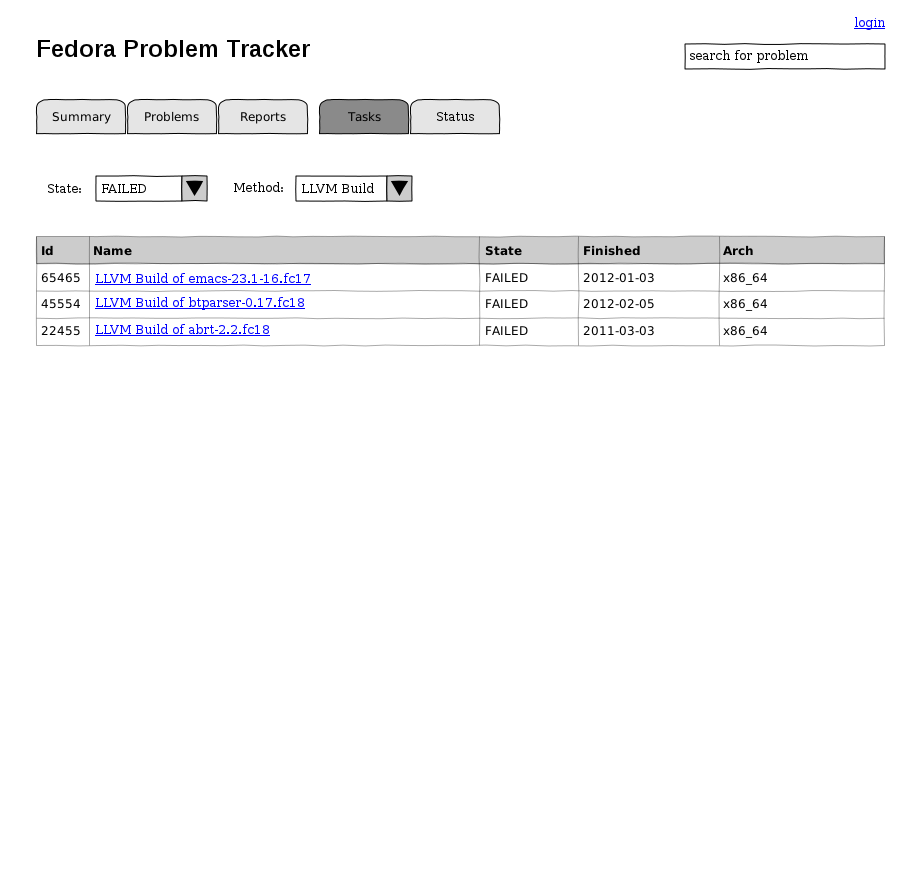
\includegraphics[width=\textwidth, trim=0 16cm 0 0, clip=true]{server-ui-tasks.png}}
\end{center}

\subsubsection{Server Status Page}
\begin{center}
\shadowbox{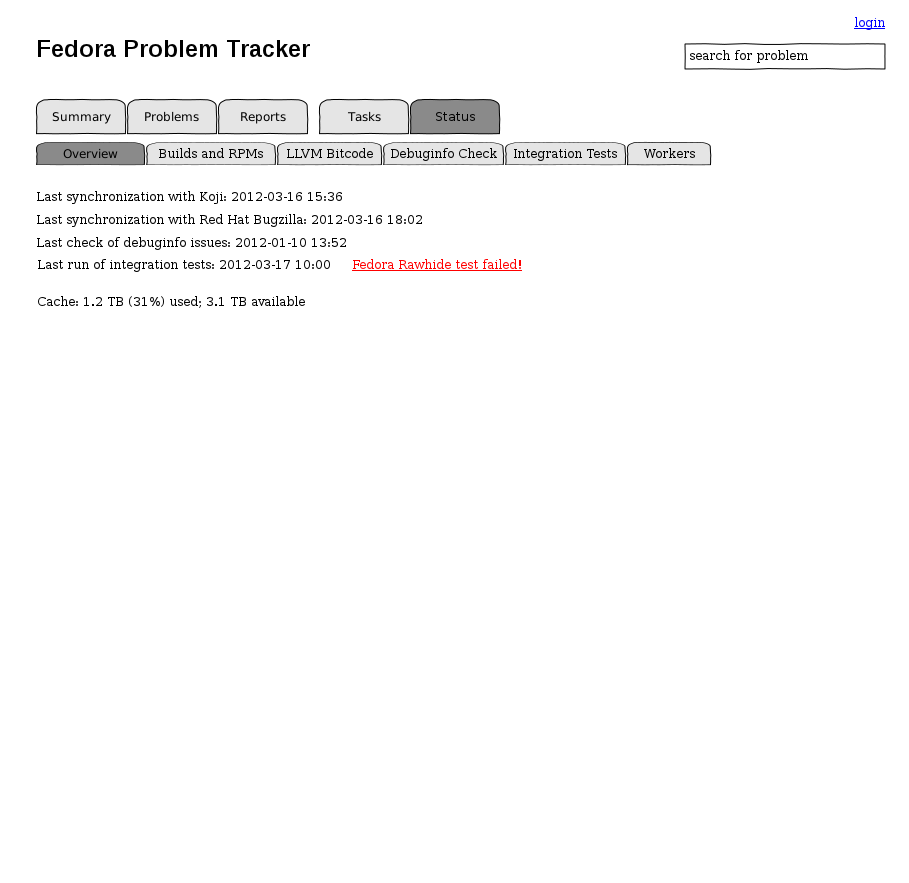
\includegraphics[width=\textwidth, trim=0 17cm 0 0, clip=true]{server-ui-status.png}}
\end{center}

\cleardoublepage
\subsubsection{Problem Reporting Interface}

Server accepts microreports.  Microreport is a JSON-formatted data
structure described below:

\begin{flushleft}
\begin{tabular}{|l|p{5cm}|c|p{5cm}|}
\hline
Name & Format & Mandatory & Notes \\ \hline
\texttt{type} & \texttt{python}, \texttt{userspace}, or \texttt{kerneloops} & yes & \\
\texttt{reason} & Unicode string, max. 128 characters. & yes & Format depends on the \texttt{type}. \\
\texttt{uptime} & Unsigned integer. & yes & Number of seconds from program start to the problem. \\
\texttt{executable} & Full path, max. 512 characters. & yes & \\
\texttt{installed\_package} & Dictionary; see the \texttt{package} table below. & yes & \\
\texttt{running\_package} & Dictionary; see the \texttt{package} table below. & no & \\
\texttt{related\_packages} & List of dictionaries; see the \texttt{related\_package} description below. & yes & \\
\texttt{os} & Dictionary; see the \texttt{os} table below. & yes & \\
\texttt{architecture} & \texttt{x86\_64} or \texttt{i386} & yes & \\
\texttt{reporter} & Dictionary; see the \texttt{reporter} table below. & yes & Program that created the report. \\
\texttt{core\_backtrace} & & yes & \\
\texttt{os\_state} & Dictionary; see the corresponding table below. & yes & \\
\texttt{user\_type} & \texttt{root}, \texttt{nologin}, \texttt{local}, or \texttt{remote} & no & \\
\texttt{selinux} & Dictionary; see the corresponding table below. & no & SELinux presence and mode. \\
\texttt{proc\_status} & ASCII string, max. 2 kB. & & The contents of \texttt{/proc/pid/status}. \\
\hline
\end{tabular}
\end{flushleft}

The \texttt{os} structure:

\begin{flushleft}
\begin{tabular}{|l|p{5cm}|c|p{5cm}|}
\hline
Name & Format & Mandatory & Notes \\ \hline
\texttt{name} & ASCII string. & yes &  \\
\texttt{version} & ASCII string & yes & Numeric. No codenames. \\
\hline
\end{tabular}
\end{flushleft}

The \texttt{os\_state} structure:

\begin{flushleft}
\begin{tabular}{|l|p{5cm}|c|p{5cm}|}
\hline
Name & Format & Mandatory & Notes \\ \hline
\texttt{suspend} & \texttt{yes} or \texttt{no} & no & Problem happened during suspend, hibernate, or resume. \\
\texttt{boot} & \texttt{yes} or \texttt{no} & no & Problem happened during boot process. \\
\texttt{login} & \texttt{yes} or \texttt{no} & no & Problem happened during login process. \\
\texttt{logout} & \texttt{yes} or \texttt{no} & no & Problem happened during logout process. \\
\texttt{shutdown} & \texttt{yes} or \texttt{no} & no & Problem happened during the shutdown process. \\
\hline
\end{tabular}
\end{flushleft}

The \texttt{reporter} structure:

\begin{flushleft}
\begin{tabular}{|l|p{5cm}|c|p{5cm}|}
\hline
Name & Format & Mandatory & Notes \\ \hline
\texttt{name} & ASCII string, max. 128 characters. & yes & \\
\texttt{version} & ASCII string, max. 128 characters. & yes & \\
\hline
\end{tabular}
\end{flushleft}

The \texttt{related\_package} structure:

\begin{flushleft}
\begin{tabular}{|l|p{5cm}|c|p{5cm}|}
\hline
Name & Format & Mandatory & Notes \\ \hline
\texttt{installed\_package} & Dictionary; see the \texttt{package} table below. & yes & \\
\texttt{running\_package} & Dictionary; see the \texttt{package} table below. & no & \\
\hline
\end{tabular}
\end{flushleft}

The \texttt{package} structure:

\begin{flushleft}
\begin{tabular}{|l|p{5cm}|c|p{5cm}|}
\hline
Name & Format & Mandatory & Notes \\ \hline
\texttt{name} & ASCII string, max. 128 characters. & yes & \\
\texttt{version} & ASCII string, max. 128 characters. & yes & \\
\texttt{release} & ASCII string, max. 128 characters. & yes & \\
\texttt{architecture} & ASCII string, max. 128 characters. & yes & \\
\texttt{epoch} & ASCII string, max. 128 characters. & yes & \\
\hline
\end{tabular}
\end{flushleft}

The \texttt{selinux} structure:

\begin{flushleft}
\begin{tabular}{|l|p{5cm}|p{3cm}|p{5cm}|}
\hline
Name & Format & Mandatory & Notes \\ \hline
\texttt{mode} & \texttt{enforcing}, \texttt{permissive}, or \texttt{disabled} & yes & \\
\texttt{context} & ASCII string, max. 128 characters & yes, if the \texttt{mode} is either \texttt{enforcing} or \texttt{permissive} & \texttt{ps -e --context} \\
\texttt{policy\_package} & Dictionary; see the \texttt{package} description. & no & \\
\hline
\end{tabular}
\end{flushleft}

\cleardoublepage
\subsubsection{Backtrace Search Interface}

Request:

\begin{flushleft}
\begin{tabular}{|l|p{5cm}|p{3cm}|p{5cm}|}
\hline
Name       & Format          & Mandatory & Notes \\
\hline
backtrace  & Unicode string. & yes       & \\
os release & ASCII string.   & yes       & \\
component  & ASCII string.   & yes       & \\
\hline
\end{tabular}
\end{flushleft}

Response:

\begin{flushleft}
\begin{tabular}{|l|p{5cm}|p{3cm}|p{5cm}|}
\hline
Name & Format & Mandatory & Notes \\
\hline
response & List of dictionaries; see the \texttt{bug} dictionary description. & Either \texttt{response} or \texttt{error} must be present. & \\
error & String. & Either \texttt{response} or \texttt{error} must be present. & \\
\hline
\end{tabular}
\end{flushleft}

\cleardoublepage
\subsubsection{Backtrace Analysis Interface}

backtrace

backtrace
thread
crash thread marked
frame
crash frame marked


\cleardoublepage
\subsubsection{Retrace Interface}

executable
os release
interactive
coredump

task id
password

\subsection{ABRT Client Overview}

\begin{center}
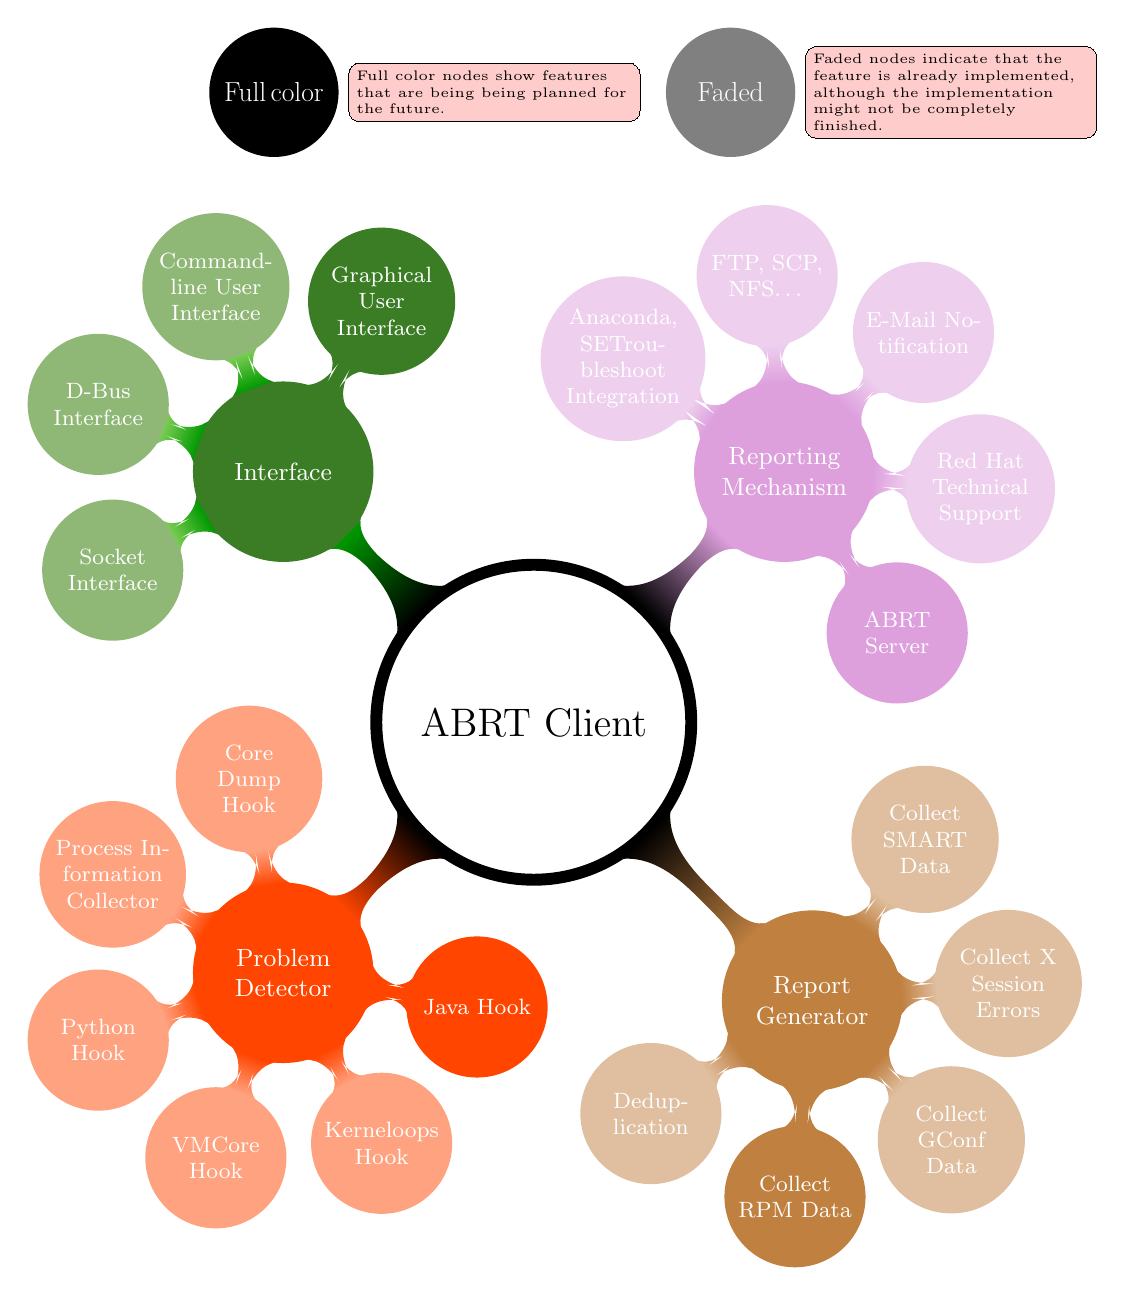
\begin{tikzpicture}[mindmap,
  every node/.style={concept},
  every annotation/.style={fill=red!20, line width=0, text=black},
  root concept/.append style={concept color=black, fill=white, line width=1ex, text=black, font=\Large},
  text=white,
  detector/.style={concept color=OrangeRed, faded/.style={concept color=OrangeRed!50}},
  generator/.style={concept color=brown, faded/.style={concept color=brown!50}},
  reporting/.style={concept color=Plum, faded/.style={concept color=Plum!50}},
  interface/.style={concept color=OliveGreen, faded/.style={concept color=OliveGreen!50}},
  grow cyclic,
  level 1/.append style={level distance=4.5cm, sibling angle=90},
  level 2/.append style={level distance=2.5cm, sibling angle=50},
  level 3/.append style={level distance=3cm, sibling angle=40}]

  \node[color=black, text=white, scale=0.4, inner sep=0pt, outer sep=0pt] (planned) at (-3.3,8) {\Huge Full color};
  \node[annotation,right] at (planned.east) {Full color nodes show
    features that are being being planned for the future.};

  \node[color=black!50, text=white, scale=0.4, inner sep=0, outer sep=0pt] (implemented) at (2.5,8) {\Huge Faded};
  \node[annotation,right] at (implemented.east) {Faded nodes indicate
    that the feature is already implemented, although the
    implementation might not be completely finished.};

  \node[root concept] {ABRT Client}
    child[detector] {node {Problem Detector}
      child[faded] {node[faded] {Core Dump Hook}}
      child[faded] {node[faded] {Process Information Collector}}
      child[faded] {node[faded] {Python Hook}}
      child[faded] {node[faded] {VMCore Hook}}
      child[faded] {node[faded] {Kerneloops Hook}}
      child {node {Java Hook}}
    }
    child[generator, level distance=5cm] {node {Report Generator}
      child[faded] {node[faded] {Dedup\-li\-ca\-tion}}
      child {node {Collect RPM Data}}
      child[faded] {node[faded] {Collect GConf Data}}
      child[faded] {node[faded] {Collect X Session Errors}}
      child[faded] {node[faded] {Collect SMART Data}}
    }
    child[reporting] {node {Reporting Mechanism}
      child {node {ABRT Server}}
      child[faded] {node[faded] {Red Hat Technical Support}}
      child[faded] {node[faded] {E-Mail Notification}}
      child[faded] {node[faded] {FTP, SCP, NFS\ldots}}
      child[faded] {node[faded] {Anaconda, SETroubleshoot Integration}}
    }
    child[interface] {node {Interface}
      child {node {Graphical User Interface}}
      child[faded] {node[faded] {Command-line User Interface}}
      child[faded] {node[faded] {D-Bus Interface}}
      child[faded] {node[faded] {Socket Interface}}
    };
\end{tikzpicture}
\end{center}

\subsection{ABRT Client Interface Overview}

\begin{center}
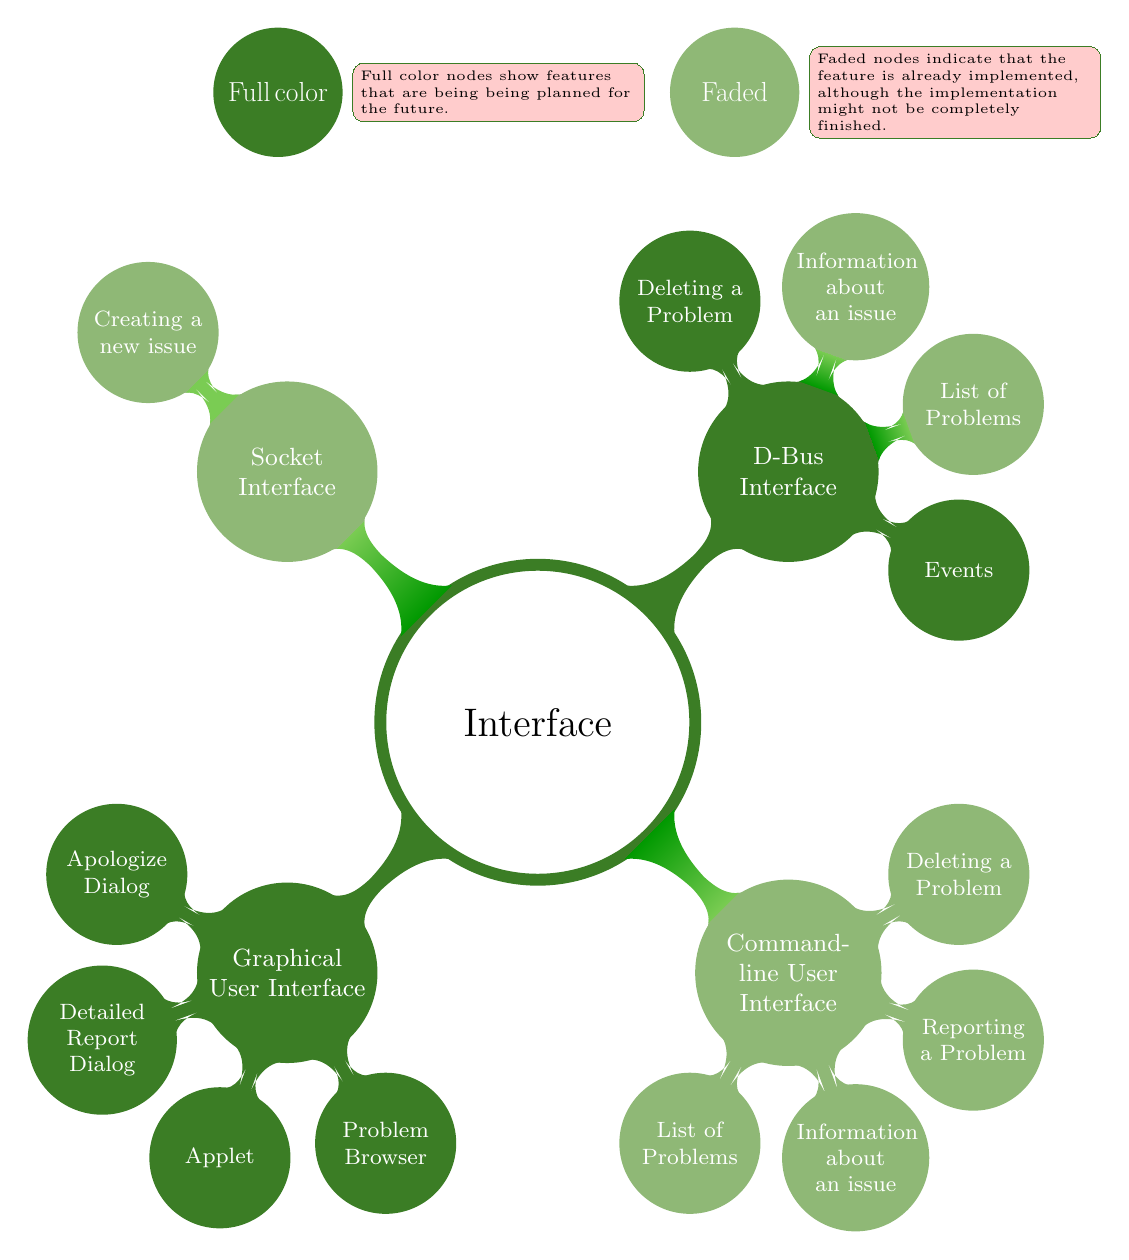
\begin{tikzpicture}[mindmap,
  every node/.style={concept, concept color=OliveGreen},
  every annotation/.style={fill=red!20, line width=0, text=black},
  faded/.style={concept color=OliveGreen!50},
  concept color=OliveGreen,
  root concept/.append style={fill=white, line width=1ex, text=black, font=\Large},
  text=white,
  grow cyclic,
  level 1/.append style={level distance=4.5cm, sibling angle=90},
  level 2/.append style={level distance=2.5cm, sibling angle=50},
  level 3/.append style={level distance=3cm, sibling angle=40}]

  \node[scale=0.4, inner sep=0pt, outer sep=0pt] (planned) at (-3.3,8) {\Huge Full color};
  \node[annotation,right] at (planned.east) {Full color nodes show
    features that are being being planned for the future.};

  \node[faded, scale=0.4, inner sep=0, outer sep=0pt] (implemented) at (2.5,8) {\Huge Faded};
  \node[annotation,right] at (implemented.east) {Faded nodes indicate
    that the feature is already implemented, although the
    implementation might not be completely finished.};

  \node[root concept] {Interface}
    child {node {Graphical User Interface}
      child {node {Apologize Dialog}}
      child {node {Detailed Report Dialog}}
      child {node {Applet}}
      child {node {Problem Browser}}
    }
    child[faded] {node[faded] {Command-line User Interface}
      child {node[faded] {List of Problems}}
      child {node[faded] {Information about an issue}}
      child {node[faded] {Reporting a Problem}}
      child {node[faded] {Deleting a Problem}}
    }
    child {node {D-Bus Interface}
      child {node {Events}}
      child[faded] {node[faded] {List of Problems}}
      child[faded] {node[faded] {Information about an issue}}
      child {node {Deleting a Problem}}
    }
    child[faded] {node[faded] {Socket Interface}
      child[faded] {node[faded] {Creating a new issue}}
    };
\end{tikzpicture}
\end{center}

\cleardoublepage
\subsubsection{Apology Dialog}
The dialogs come from \cite{JonOops}. Please see \cite{JonOops} for
more detailed design.

\begin{center}
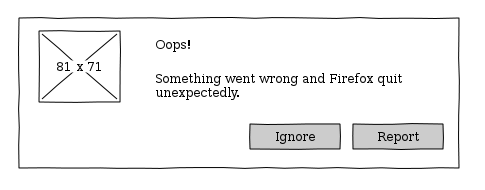
\includegraphics[width=\textwidth]{client-ui-apology-dialog-manual.png}
\end{center}

\begin{center}
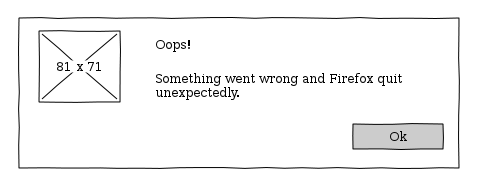
\includegraphics[width=\textwidth]{client-ui-apology-dialog-automatic.png}
\end{center}

\subsubsection{Detailed Report Dialog}
\begin{center}
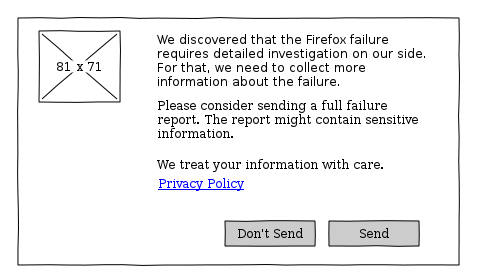
\includegraphics[width=\textwidth]{client-ui-detailed-report-dialog.png}
\end{center}

\subsubsection{Applet}

\cleardoublepage
\subsubsection{Problem Browser}
The Problem Browser dialog comes from \cite{JonOops}. Please see
\cite{JonOops} for more detailed design.

\begin{center}
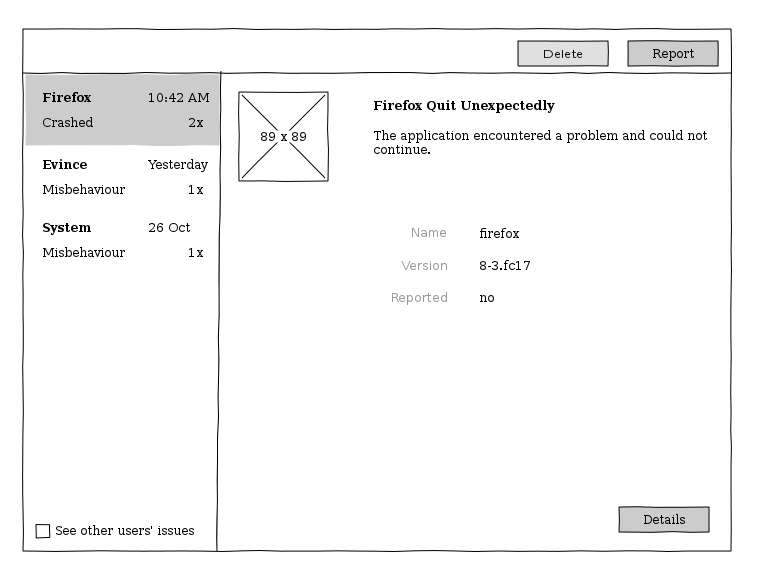
\includegraphics[width=\textwidth]{client-ui-issue-browser.png}
\end{center}

\subsection{ABRT Client Reporting Mechanism Overview}

\subsubsection{Reporting to ABRT Server}

\subsection{ABRT Client Report Generator Overview}

\subsubsection{Coredump-level backtraces}




\cleardoublepage
\section{Project Time Management}

\subsection{Fedora 17 Phase}
Finish date: approx 2012-06-01. \\
Consists of 3 sprints, 3 weeks each. \\

The goals for the ABRT Server to be reached at the end of the
phase:

\begin{description}
\item[Usable human user interface] Server has initial but usable
  graphical user interface.  It shows problems, reports, and report
  history in a graph.
\item[$\mu$Report processing] Server accepts $\mu$reports, stores them
  to the database, retraces the contained symbols.  Accepted reports
  are visible in the user interface.
\item[Clustering of reports into problems] Report clusters (problems)
  on server are generated using core-backtrace distance.
\end{description}

The goals for the ABRT Client to be reached at the end of the phase:
\begin{description}
\item[$\mu$Report sending] Client sends $\mu$reports from the crash
  dialog.
\end{description}

\cleardoublepage
\subsubsection{Sprint 1}
Finish date: 2012-03-20 Tuesday \\
Duration: 3 weeks \\
Status: FINISHED

\begin{itemize}
\item Server
  \begin{itemize}
  \item Problem storage
    \begin{itemize}
    \item Database schema [mtoman,mlichvar]
    \item Storage of incoming problems [mlichvar]
    \end{itemize}
  \item Data storage
    \item Initial database schema [mtoman]
  \item Deduplication
    \begin{itemize}
    \item Deduplication of incoming problems according to hashes
    \item Deduplication of retraced problems according to symbols
    \end{itemize}
  \item Retracing
    \begin{itemize}
    \item Retracing of microreports
    \end{itemize}
  \item Machine interface
    \begin{itemize}
    \item Receive report
    \end{itemize}
  \item Migration to SQLAlchemy [mlichvar]
  \item RHEL6 compatibility [mtoman]
  \end{itemize}
\item Client
  \begin{itemize}
  \item Coredump-level backtraces [mmilata]
  \item Microreport sender [npajkovs]
  \item User interface [dvlasenk]
  \end{itemize}
\end{itemize}

\cleardoublepage
\subsubsection{Sprint 2}
Start date: 2012-04-02 Monday \\
Finish date: 2012-04-27 Friday \\
Duration: approx. 3 weeks

\begin{itemize}
\item Server
  \begin{itemize}
  \item Human interface
  \item Machine interface
  \item Tasks and workers
  \item Clustering
    \begin{itemize}
      \item Adapt existing source code to match the server
      \item Properly create problems from reports
    \end{itemize}
  \end{itemize}
\end{itemize}

\cleardoublepage
\subsubsection{Sprint 3}
Start date: 2012-05-07 Monday \\
Finish date: approx. 2012-06-01 Friday \\
Duration: approx. 4 weeks

\begin{itemize}
\item Accepting reports on the server
\item Python and Koops $\mu$reports
\item Rewrite cache to storage
\item Generating problems
\item Deploy server internally
\end{itemize}

\cleardoublepage
\subsection{Fedora 18 Phase}
Finish date: approx. 2012-11-01


The goals for the ABRT Server to be reached at the end of the
phase:
\begin{description}
\item[Retrace server merged] Retrace server functionality is merged
  into the server, using server's packages, server's \textit{chroot}
  implementation and server's \textit{libsolv} integration.  The
  original retrace server is still maintained to support current
  deployments.
\item[Debuginfo check] Server checks the consistency of packages
  containing the debugging symbols for program binaries.  It supports
  opening bugs for packages with broken debugging symbols.
\item[LLVM support] Server handles LLVM rebuilds of packages to allow
  static analysis of source code and source code browser.
\item[Full reports] Server requests and stores full report (coredump)
  for problems that require fixing due to high priority.
\item[Better human interface] Problems and reports can be studied by
  users in a good detail.  Server shows its status (which packages are
  supported, internal task failures such as failed package download or
  LLVM rebuild).
\item[Machine interface] Problems and reports can be fetched via
  JSON. Problems, reports, and Red Hat Bugzilla bugs can be searched
  by providing a backtrace.  Server can be used to obtain the crash
  function from a textual backtrace.
\end{description}

The goals for the ABRT Client to be reached at the end of the phase:
\begin{description}
\item[Better human interface]
\end{description}

\cleardoublepage
\subsubsection{Sprint 4}
Start date: approx.
Duration: approx. 3 weeks

\begin{itemize}
\item Determine crash function from core backtrace
\item Problem names and report names
\item Finish retracing
\item JSON interface for search with a backtrace
\item LLVM rebuild
\item Builds and packages page in Status
\item Overview page in Status
\item RHBZ Bugs in Status
\end{itemize}

\cleardoublepage
\subsubsection{Sprint 5}
Duration: approx. 3 weeks

\begin{itemize}
\item Extend LLVM rebuild with DXR for source code browsing.
\item Interface for source code browsing (clickable function names in
  coredump-level backtraces.
\item Request and store coredumps and vmcores.
\item Implement coredump and vmcore retracing.
\item JSON API for coredump and vmcore retracing.
\end{itemize}

\cleardoublepage
\subsubsection{Sprint 6}
Duration: approx. 3 weeks

\begin{itemize}
\item LLVM linking into single module
\item Component groups
\item Debuginfo checker
\end{itemize}

\cleardoublepage
\subsubsection{Sprint 7}
Duration: approx. 3 weeks

\begin{itemize}
\item Problem type analysis start
\item Security analysis start
\item Merge All/Running/Finished Tasks in Status into single page.
\item Debuginfo checker integration with brewtap
\end{itemize}

\cleardoublepage
\subsubsection{Sprint 8}
Duration: approx. 3 weeks

\begin{itemize}
\item Bugfixing
\item Fedora deployment
\end{itemize}

\cleardoublepage
\subsection{Fedora 19 Phase}

The goals for the ABRT Server to be reached at the end of the
phase:
\begin{description}
\item[Automatic reporting to Red Hat Bugzilla]
\item[Security analysis of reports]
\item[Static analysis of SELinux AVCs]
\end{description}

\cleardoublepage
\subsubsection{Sprint 9}
\begin{itemize}
\item SELinux AVCs
\item Reporting to Red Hat Bugzilla
\end{itemize}

\cleardoublepage
\subsubsection{Sprint 10 and later}
\begin{itemize}
\item Reporting to upstreams
\item SELinux analysis
\item Symbolic execution
\item Crash analysis
\end{itemize}


%\subsection{Activity List}
%\begin{enumerate}
%\item Set-up and document regular, automatic database backup. [server]
%\item Finish the design of minireport and fullreport backup. [server]
%\item Implement minireport and fullreport backup. [server]
%\item Implement deduplication logic on arrival of a new report. [server]
%\item Implement deduplication logic for clustering and merging of
%  existing reports. [server]
%\item Implement coredump-level backtraces. [server]
%\item Implement retracing of coredump-level backtraces. [server]
%\item Implement both variants of apology dialog. [client]
%\item Implement detailed report dialog. [client]
%\end{enumerate}
%- Define Activities
%-- Activity List
%-- Activity attributes
%-- Milestone list
%
%- Sequence Activities
%-- Project Schedule Network Diagram
%
%- Estimate Activity Resources
%-- Activity Resource Requirements
%-- Resource Breakdown Structure
%- Estimate Activity Durations
%-- Activity Duration Estimates
%- Develop Schedule
%-- Project Schedule
%-- Schedule baseline
%-- Schedule data
%\section{Project Cost Management}
%- Estimate Costs
%-- Activity Cost Estimates
%-- Basis of estimates
%- Determine Budget
%-- Cost performance baseline
%-- Project funding requirements

%\cleardoublepage
%\section{Project Quality Management}
%- Plan Quality
%-- Quality management plan
%-- Quality metrics
%-- Quality checklists
%-- Process improvement plan

%\section{Project Human Resource Management}

%- Develop Human Resource Plan

%\section{Project Communications Management}

%- Plan Communications

%\cleardoublepage
%\section{Project Risk Management}

%Plan Risk Management
%-- Risk Register

%Identify Risks

%Perform Qualitative Risk Analysis

%Perform Quantitative Risk Analysis

%Plan Risk Responses

%\cleardoublepage
%\section{Project Management Plan}


\cleardoublepage
\section{Related Work}
There are several existing implementations of software failure
management systems.

\subsection{GNOME Problem Reporting}
Jon McCann of GNOME team envisioned a problem reporting
architecture\cite{JonProposal} that splits the responsibilities of a
problem management system into several components:
\begin{enumerate}
\item \emph{System Logger} collects data for anomalous behavior of
  system such as crash dumps and SELinux access denial logs.  It is
  proposed to include this functionality into \texttt{systemd}, a
  system and service manager for Linux.  In internal communication,
  Jon also proposed to stop using core dumps in favor of minidumps.
\item \emph{Problem Detector} watches the output of System Logger for
  new events, and runs Report Generator on every new event.  Its name
  should be \texttt{problemd}, and this tool is not implemented yet.
\item \emph{Report Generator} gathers supplementary details about a
  problem, and stores problem data to a non-volatile memory.  It
  should be handled by either \texttt{systemd} or \texttt{problemd}.
\item \emph{User Problem Notifier} notifies user about a problem.  Jon
  proposes to include this functionality into
  \texttt{gnome-settings-daemon}.
\item \emph{Reporting Mechanism} delivers problem report to a
  Collection Server, scp, ftp, email\ldots
\item \emph{Problem Reporting and Review} shows problem reports of a
  system, and allows report submission.  Jon designed
  \emph{Oops!}\cite{JonOops}, a graphical user interface for such a
  component.
\item \emph{Problem Report Collection Server} accepts anonymous
  submissions, supports filling reports to Bugzilla, scrubs sensitive
  data from reports, detects duplicates, performs coredump analysis
  and retracing (generating backtrace from coredump).  In internal
  communication, GNOME team proposes using
  \href{https://wiki.mozilla.org/Socorro}{Socorro}, a crash statistics
  server project of Mozilla, in this role.
\end{enumerate}

\paragraph{Advantages and good aspects of the proposal.}
\begin{enumerate}
\item The idea of pushing generic code to packages that are being used
  across distributions.  Coredump catching can definitely be done by
  \texttt{systemd}. \emph{Problem Detector} and \emph{Report
    Generator} can also be made portable and shareable across
  distributions, and it could live in \url{http://freedesktop.org} as
  \texttt{problemd}.
\item The design of \emph{Oops!}.
\end{enumerate}

\paragraph{Criticism of the proposal.}
\begin{figure}[h!]
\centering
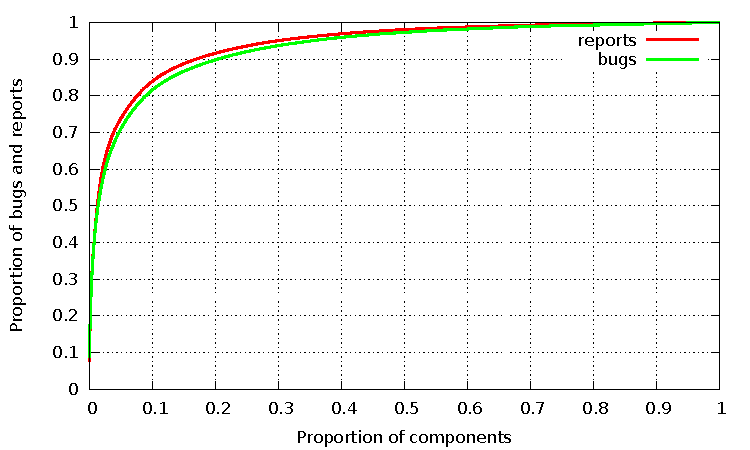
\includegraphics[width=0.8\textwidth]{abrt-bugs-per-component-cdf.pdf}
\caption{Cumulative distribution of ABRT bugs and reports per
  component}
\label{fig:cumulative}
\end{figure}

\begin{figure}[h!]
\centering
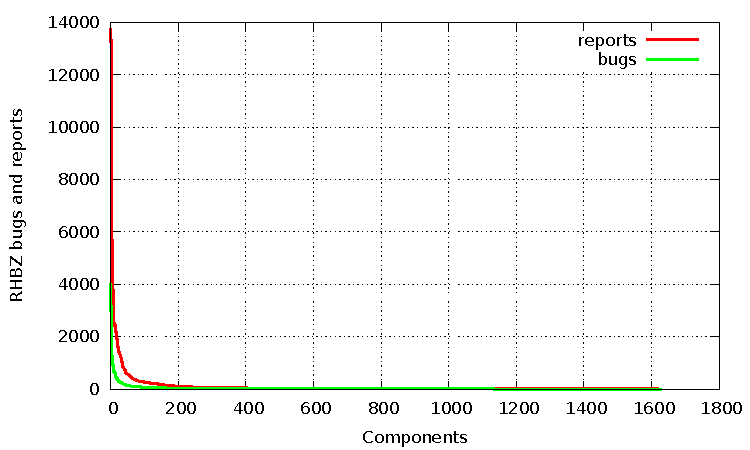
\includegraphics[width=0.8\textwidth]{abrt-bugs-per-component.pdf}
\caption{Distribution of ABRT bugs and reports per component}
\label{fig:distribution}
\end{figure}

The most important point that should be re-evaluated is the proposed
direction of \emph{statistics-based} problem management and
bugfixing. This includes the usage of minidumps in all situations, and
the deployment of Socorro.

Data from the current problem management system shows that
statistics-based bugfixing misfits the operating system level use case
(management of full stack of applications).  Statistics-based
bugfixing is based on the assumption of large amounts of users hitting
and reporting the same crash.  This assumption is valid for desktop
applications, which are quickly changing, contain large amount of bugs
(GUI code is difficult to handle well), and have large amount of users
(desktop shell, internet browser, e-mail client).  Nevertheless, this
assumption is \emph{invalid} for most of operating system packages,
including server-side software. Many packages are used by relatively
low number of people, customized and deployed just on a few servers.
Crashes in this situation are less frequent, but dangerous.

\begin{enumerate}
\item Implementing \emph{User Problem Notifier} into
  \texttt{gnome-settings-daemon} brings the requirement to implement
  the same functionality for other desktops as well (KDE, XFCE).
\item \emph{Oops!} design is incomplete. It is not clear how the
  reporting target can be configured (problem report collection server
  URL, e-mail, FTP, SCP destinations).  The window with report details
  is not presented.
\end{enumerate}

\subsection{Windows Error Reporting}
TODO: \cite{MS}.

\subsection{Ubuntu Apport}


\cleardoublepage
\begin{thebibliography}{9}

\bibitem{JonOops}
  Jon McCann,
  \emph{Oops!}.
  \url{https://live.gnome.org/Design/Apps/Oops}.

\bibitem{JonOverview}
  Jon McCann,
  \emph{Problem Recovery and Reporting}.
  \url{https://live.gnome.org/GnomeOS/Design/Whiteboards/ProblemReporting}.

\bibitem{JonProposal}
  Jon McCann,
  \emph{Problem Reporting Architecture Proposal}.
  \url{https://live.gnome.org/GnomeOS/Design/Whiteboards/ProblemReporting/Proposal}.

\bibitem{MS}
  \emph{Debugging in the (Very) Large: Ten Years of Implementation and Experience}.
  \url{http://msdn.microsoft.com/en-us/windows/hardware/gg487440}.

\end{thebibliography}

\end{document}
